% Options for packages loaded elsewhere
\PassOptionsToPackage{unicode}{hyperref}
\PassOptionsToPackage{hyphens}{url}
\PassOptionsToPackage{dvipsnames,svgnames,x11names}{xcolor}
%
\documentclass[
  11pt,
  letterpaper,
  DIV=11,
  numbers=noendperiod]{scrartcl}

\usepackage{amsmath,amssymb}
\usepackage{setspace}
\usepackage{iftex}
\ifPDFTeX
  \usepackage[T1]{fontenc}
  \usepackage[utf8]{inputenc}
  \usepackage{textcomp} % provide euro and other symbols
\else % if luatex or xetex
  \usepackage{unicode-math}
  \defaultfontfeatures{Scale=MatchLowercase}
  \defaultfontfeatures[\rmfamily]{Ligatures=TeX,Scale=1}
\fi
\usepackage{lmodern}
\ifPDFTeX\else  
    % xetex/luatex font selection
\fi
% Use upquote if available, for straight quotes in verbatim environments
\IfFileExists{upquote.sty}{\usepackage{upquote}}{}
\IfFileExists{microtype.sty}{% use microtype if available
  \usepackage[]{microtype}
  \UseMicrotypeSet[protrusion]{basicmath} % disable protrusion for tt fonts
}{}
\makeatletter
\@ifundefined{KOMAClassName}{% if non-KOMA class
  \IfFileExists{parskip.sty}{%
    \usepackage{parskip}
  }{% else
    \setlength{\parindent}{0pt}
    \setlength{\parskip}{6pt plus 2pt minus 1pt}}
}{% if KOMA class
  \KOMAoptions{parskip=half}}
\makeatother
\usepackage{xcolor}
\usepackage[margin = 1in]{geometry}
\setlength{\emergencystretch}{3em} % prevent overfull lines
\setcounter{secnumdepth}{-\maxdimen} % remove section numbering
% Make \paragraph and \subparagraph free-standing
\ifx\paragraph\undefined\else
  \let\oldparagraph\paragraph
  \renewcommand{\paragraph}[1]{\oldparagraph{#1}\mbox{}}
\fi
\ifx\subparagraph\undefined\else
  \let\oldsubparagraph\subparagraph
  \renewcommand{\subparagraph}[1]{\oldsubparagraph{#1}\mbox{}}
\fi

\usepackage{color}
\usepackage{fancyvrb}
\newcommand{\VerbBar}{|}
\newcommand{\VERB}{\Verb[commandchars=\\\{\}]}
\DefineVerbatimEnvironment{Highlighting}{Verbatim}{commandchars=\\\{\}}
% Add ',fontsize=\small' for more characters per line
\usepackage{framed}
\definecolor{shadecolor}{RGB}{241,243,245}
\newenvironment{Shaded}{\begin{snugshade}}{\end{snugshade}}
\newcommand{\AlertTok}[1]{\textcolor[rgb]{0.68,0.00,0.00}{#1}}
\newcommand{\AnnotationTok}[1]{\textcolor[rgb]{0.37,0.37,0.37}{#1}}
\newcommand{\AttributeTok}[1]{\textcolor[rgb]{0.40,0.45,0.13}{#1}}
\newcommand{\BaseNTok}[1]{\textcolor[rgb]{0.68,0.00,0.00}{#1}}
\newcommand{\BuiltInTok}[1]{\textcolor[rgb]{0.00,0.23,0.31}{#1}}
\newcommand{\CharTok}[1]{\textcolor[rgb]{0.13,0.47,0.30}{#1}}
\newcommand{\CommentTok}[1]{\textcolor[rgb]{0.37,0.37,0.37}{#1}}
\newcommand{\CommentVarTok}[1]{\textcolor[rgb]{0.37,0.37,0.37}{\textit{#1}}}
\newcommand{\ConstantTok}[1]{\textcolor[rgb]{0.56,0.35,0.01}{#1}}
\newcommand{\ControlFlowTok}[1]{\textcolor[rgb]{0.00,0.23,0.31}{#1}}
\newcommand{\DataTypeTok}[1]{\textcolor[rgb]{0.68,0.00,0.00}{#1}}
\newcommand{\DecValTok}[1]{\textcolor[rgb]{0.68,0.00,0.00}{#1}}
\newcommand{\DocumentationTok}[1]{\textcolor[rgb]{0.37,0.37,0.37}{\textit{#1}}}
\newcommand{\ErrorTok}[1]{\textcolor[rgb]{0.68,0.00,0.00}{#1}}
\newcommand{\ExtensionTok}[1]{\textcolor[rgb]{0.00,0.23,0.31}{#1}}
\newcommand{\FloatTok}[1]{\textcolor[rgb]{0.68,0.00,0.00}{#1}}
\newcommand{\FunctionTok}[1]{\textcolor[rgb]{0.28,0.35,0.67}{#1}}
\newcommand{\ImportTok}[1]{\textcolor[rgb]{0.00,0.46,0.62}{#1}}
\newcommand{\InformationTok}[1]{\textcolor[rgb]{0.37,0.37,0.37}{#1}}
\newcommand{\KeywordTok}[1]{\textcolor[rgb]{0.00,0.23,0.31}{#1}}
\newcommand{\NormalTok}[1]{\textcolor[rgb]{0.00,0.23,0.31}{#1}}
\newcommand{\OperatorTok}[1]{\textcolor[rgb]{0.37,0.37,0.37}{#1}}
\newcommand{\OtherTok}[1]{\textcolor[rgb]{0.00,0.23,0.31}{#1}}
\newcommand{\PreprocessorTok}[1]{\textcolor[rgb]{0.68,0.00,0.00}{#1}}
\newcommand{\RegionMarkerTok}[1]{\textcolor[rgb]{0.00,0.23,0.31}{#1}}
\newcommand{\SpecialCharTok}[1]{\textcolor[rgb]{0.37,0.37,0.37}{#1}}
\newcommand{\SpecialStringTok}[1]{\textcolor[rgb]{0.13,0.47,0.30}{#1}}
\newcommand{\StringTok}[1]{\textcolor[rgb]{0.13,0.47,0.30}{#1}}
\newcommand{\VariableTok}[1]{\textcolor[rgb]{0.07,0.07,0.07}{#1}}
\newcommand{\VerbatimStringTok}[1]{\textcolor[rgb]{0.13,0.47,0.30}{#1}}
\newcommand{\WarningTok}[1]{\textcolor[rgb]{0.37,0.37,0.37}{\textit{#1}}}

\providecommand{\tightlist}{%
  \setlength{\itemsep}{0pt}\setlength{\parskip}{0pt}}\usepackage{longtable,booktabs,array}
\usepackage{calc} % for calculating minipage widths
% Correct order of tables after \paragraph or \subparagraph
\usepackage{etoolbox}
\makeatletter
\patchcmd\longtable{\par}{\if@noskipsec\mbox{}\fi\par}{}{}
\makeatother
% Allow footnotes in longtable head/foot
\IfFileExists{footnotehyper.sty}{\usepackage{footnotehyper}}{\usepackage{footnote}}
\makesavenoteenv{longtable}
\usepackage{graphicx}
\makeatletter
\def\maxwidth{\ifdim\Gin@nat@width>\linewidth\linewidth\else\Gin@nat@width\fi}
\def\maxheight{\ifdim\Gin@nat@height>\textheight\textheight\else\Gin@nat@height\fi}
\makeatother
% Scale images if necessary, so that they will not overflow the page
% margins by default, and it is still possible to overwrite the defaults
% using explicit options in \includegraphics[width, height, ...]{}
\setkeys{Gin}{width=\maxwidth,height=\maxheight,keepaspectratio}
% Set default figure placement to htbp
\makeatletter
\def\fps@figure{htbp}
\makeatother
% definitions for citeproc citations
\NewDocumentCommand\citeproctext{}{}
\NewDocumentCommand\citeproc{mm}{%
  \begingroup\def\citeproctext{#2}\cite{#1}\endgroup}
\makeatletter
 % allow citations to break across lines
 \let\@cite@ofmt\@firstofone
 % avoid brackets around text for \cite:
 \def\@biblabel#1{}
 \def\@cite#1#2{{#1\if@tempswa , #2\fi}}
\makeatother
\newlength{\cslhangindent}
\setlength{\cslhangindent}{1.5em}
\newlength{\csllabelwidth}
\setlength{\csllabelwidth}{3em}
\newenvironment{CSLReferences}[2] % #1 hanging-indent, #2 entry-spacing
 {\begin{list}{}{%
  \setlength{\itemindent}{0pt}
  \setlength{\leftmargin}{0pt}
  \setlength{\parsep}{0pt}
  % turn on hanging indent if param 1 is 1
  \ifodd #1
   \setlength{\leftmargin}{\cslhangindent}
   \setlength{\itemindent}{-1\cslhangindent}
  \fi
  % set entry spacing
  \setlength{\itemsep}{#2\baselineskip}}}
 {\end{list}}
\usepackage{calc}
\newcommand{\CSLBlock}[1]{\hfill\break\parbox[t]{\linewidth}{\strut\ignorespaces#1\strut}}
\newcommand{\CSLLeftMargin}[1]{\parbox[t]{\csllabelwidth}{\strut#1\strut}}
\newcommand{\CSLRightInline}[1]{\parbox[t]{\linewidth - \csllabelwidth}{\strut#1\strut}}
\newcommand{\CSLIndent}[1]{\hspace{\cslhangindent}#1}

\KOMAoption{captions}{tableheading}
\usepackage{amsmath}
\usepackage{bbm}
\usepackage{array}
\usepackage{multirow}
\usepackage{graphicx}
\usepackage{float}
\usepackage{apacite}
\usepackage{natbib}
\makeatletter
\@ifpackageloaded{caption}{}{\usepackage{caption}}
\AtBeginDocument{%
\ifdefined\contentsname
  \renewcommand*\contentsname{Table of contents}
\else
  \newcommand\contentsname{Table of contents}
\fi
\ifdefined\listfigurename
  \renewcommand*\listfigurename{List of Figures}
\else
  \newcommand\listfigurename{List of Figures}
\fi
\ifdefined\listtablename
  \renewcommand*\listtablename{List of Tables}
\else
  \newcommand\listtablename{List of Tables}
\fi
\ifdefined\figurename
  \renewcommand*\figurename{Figure}
\else
  \newcommand\figurename{Figure}
\fi
\ifdefined\tablename
  \renewcommand*\tablename{Table}
\else
  \newcommand\tablename{Table}
\fi
}
\@ifpackageloaded{float}{}{\usepackage{float}}
\floatstyle{ruled}
\@ifundefined{c@chapter}{\newfloat{codelisting}{h}{lop}}{\newfloat{codelisting}{h}{lop}[chapter]}
\floatname{codelisting}{Listing}
\newcommand*\listoflistings{\listof{codelisting}{List of Listings}}
\makeatother
\makeatletter
\makeatother
\makeatletter
\@ifpackageloaded{caption}{}{\usepackage{caption}}
\@ifpackageloaded{subcaption}{}{\usepackage{subcaption}}
\makeatother
\ifLuaTeX
  \usepackage{selnolig}  % disable illegal ligatures
\fi
\usepackage{bookmark}

\IfFileExists{xurl.sty}{\usepackage{xurl}}{} % add URL line breaks if available
\urlstyle{same} % disable monospaced font for URLs
\hypersetup{
  pdftitle={STATS 3DA3},
  pdfauthor={Lily Seebach (400331131)},
  colorlinks=true,
  linkcolor={blue},
  filecolor={Maroon},
  citecolor={Blue},
  urlcolor={Blue},
  pdfcreator={LaTeX via pandoc}}

\title{STATS 3DA3}
\usepackage{etoolbox}
\makeatletter
\providecommand{\subtitle}[1]{% add subtitle to \maketitle
  \apptocmd{\@title}{\par {\large #1 \par}}{}{}
}
\makeatother
\subtitle{Homework Assignment 6}
\author{Lily Seebach (400331131)}
\date{2024-04-18}

\begin{document}
\maketitle

\setstretch{1.5}
\newpage

\begin{enumerate}
\def\labelenumi{\arabic{enumi}.}
\item
  A classification problem based on the dataset by Rubini,
  Soundarapandian, and Eswaran (2015) is to classify an individual into
  has or doesn't have chronic kidney disease based on the following
  predictor variables: age, blood pressure (mm/Hg), specific gravity,
  albumin, sugar, red blood cells, pus cell, pus cell clumps, bacteria,
  blood glucose random (mgs/dl), blood urea (mgs/dl), serum creatinine
  (mgs/dl), sodium (mEq/L), potassium (mEq/L), hemoglobin (gms), packed
  cell volume, white blood cell count (cells/cmm), red blood cell count
  (millions/cmm), hypertension, diabetes mellitus, coronary artery
  disease, appetite, pedal edema, and anemia.
\item
  We import the data and transform it as necessary.
\end{enumerate}

\begin{Shaded}
\begin{Highlighting}[]
\ImportTok{import}\NormalTok{ pandas }\ImportTok{as}\NormalTok{ pd}
\ImportTok{import}\NormalTok{ numpy }\ImportTok{as}\NormalTok{ np}
\ImportTok{from}\NormalTok{ ucimlrepo }\ImportTok{import}\NormalTok{ fetch\_ucirepo }
\ImportTok{import}\NormalTok{ certifi}
\NormalTok{chronic\_kidney\_disease }\OperatorTok{=}\NormalTok{ fetch\_ucirepo(}\BuiltInTok{id}\OperatorTok{=}\DecValTok{336}\NormalTok{) }
\NormalTok{X }\OperatorTok{=}\NormalTok{ chronic\_kidney\_disease.data.features }
\NormalTok{y }\OperatorTok{=}\NormalTok{ chronic\_kidney\_disease.data.targets}
\NormalTok{data }\OperatorTok{=}\NormalTok{ pd.concat([X, y], axis }\OperatorTok{=} \DecValTok{1}\NormalTok{)}
\end{Highlighting}
\end{Shaded}

To check if any variable transformations are necessary, we check that
the data types of the variables in the dataframe match the description
in the data dictionary.

\begin{Shaded}
\begin{Highlighting}[]
\BuiltInTok{print}\NormalTok{(data.dtypes)}
\end{Highlighting}
\end{Shaded}

\begin{verbatim}
age      float64
bp       float64
sg       float64
al       float64
su       float64
rbc       object
pc        object
pcc       object
ba        object
bgr      float64
bu       float64
sc       float64
sod      float64
pot      float64
hemo     float64
pcv      float64
wbcc     float64
rbcc     float64
htn       object
dm        object
cad       object
appet     object
pe        object
ane       object
class     object
dtype: object
\end{verbatim}

We can see that age, blood pressure (bp), blood glucose random (bgr),
blood urea (bu), serum creatinine (sc), sodium (sod), potassium (pot),
hemoglobin (hemo), packed cell volume (pcv), white blood cell count
(wbcc), and red blood cell count (rbcc) are all numerical values as they
should be according to the data dictionary (note the data dictionary
differentiates between integer and continuous values but changing
numeric data types will not affect results). However, specific gravity
(sg), albumin (al), and sugar (su) should be nominal but are float
values. Red blood cells (rbc), pus cell (pc), pus cell clumps (pcc),
bacteria (ba), hypertension (htn), diabetes mellitus (dm), coronary
artery disease (cad), appette (appet), pedal edema (pe), anemia (ane),
and class should all be nominal instead of object as they appear now. We
correct the data type errors by converting the noted variables to
categorical/nominal.

\begin{Shaded}
\begin{Highlighting}[]
\NormalTok{columns\_to\_convert }\OperatorTok{=}\NormalTok{ [}\StringTok{\textquotesingle{}sg\textquotesingle{}}\NormalTok{,}\StringTok{\textquotesingle{}al\textquotesingle{}}\NormalTok{,}\StringTok{\textquotesingle{}su\textquotesingle{}}\NormalTok{,}\StringTok{\textquotesingle{}rbc\textquotesingle{}}\NormalTok{,}\StringTok{\textquotesingle{}pc\textquotesingle{}}\NormalTok{,}\StringTok{\textquotesingle{}pcc\textquotesingle{}}\NormalTok{,}\StringTok{\textquotesingle{}ba\textquotesingle{}}\NormalTok{,}\StringTok{\textquotesingle{}htn\textquotesingle{}}\NormalTok{,}\StringTok{\textquotesingle{}dm\textquotesingle{}}\NormalTok{,}\StringTok{\textquotesingle{}cad\textquotesingle{}}\NormalTok{,}\StringTok{\textquotesingle{}appet\textquotesingle{}}\NormalTok{,}\StringTok{\textquotesingle{}pe\textquotesingle{}}\NormalTok{,}\StringTok{\textquotesingle{}ane\textquotesingle{}}\NormalTok{,}\StringTok{\textquotesingle{}class\textquotesingle{}}\NormalTok{]}
\ControlFlowTok{for}\NormalTok{ col }\KeywordTok{in}\NormalTok{ columns\_to\_convert:}
\NormalTok{    data[col] }\OperatorTok{=}\NormalTok{ pd.Categorical(data[col])}
\end{Highlighting}
\end{Shaded}

In order to make the variables match the abbreviations found in the data
dictionary, we rename wbcc and rbcc to wc and rc, respectively.

\begin{Shaded}
\begin{Highlighting}[]
\NormalTok{data }\OperatorTok{=}\NormalTok{ data.rename(columns}\OperatorTok{=}\NormalTok{\{}\StringTok{\textquotesingle{}wbcc\textquotesingle{}}\NormalTok{:}\StringTok{\textquotesingle{}wc\textquotesingle{}}\NormalTok{\})}
\NormalTok{data }\OperatorTok{=}\NormalTok{ data.rename(columns}\OperatorTok{=}\NormalTok{\{}\StringTok{\textquotesingle{}rbcc\textquotesingle{}}\NormalTok{:}\StringTok{\textquotesingle{}rc\textquotesingle{}}\NormalTok{\})}
\end{Highlighting}
\end{Shaded}

\begin{enumerate}
\def\labelenumi{\arabic{enumi}.}
\setcounter{enumi}{2}
\tightlist
\item
  We explore the data and give a detailed description of the dataset.
\end{enumerate}

\begin{Shaded}
\begin{Highlighting}[]
\BuiltInTok{print}\NormalTok{(data.shape)}
\BuiltInTok{print}\NormalTok{(data.iloc[}\DecValTok{0}\NormalTok{:}\DecValTok{2}\NormalTok{,}\DecValTok{0}\NormalTok{:}\DecValTok{12}\NormalTok{])}
\BuiltInTok{print}\NormalTok{(data.iloc[}\DecValTok{0}\NormalTok{:}\DecValTok{2}\NormalTok{,}\DecValTok{12}\NormalTok{:}\DecValTok{26}\NormalTok{])}
\end{Highlighting}
\end{Shaded}

\begin{verbatim}
(400, 25)
    age    bp    sg   al   su  rbc      pc         pcc          ba    bgr  \
0  48.0  80.0  1.02  1.0  0.0  NaN  normal  notpresent  notpresent  121.0   
1   7.0  50.0  1.02  4.0  0.0  NaN  normal  notpresent  notpresent    NaN   

     bu   sc  
0  36.0  1.2  
1  18.0  0.8  
   sod  pot  hemo   pcv      wc   rc  htn   dm cad appet  pe ane class
0  NaN  NaN  15.4  44.0  7800.0  5.2  yes  yes  no  good  no  no   ckd
1  NaN  NaN  11.3  38.0  6000.0  NaN   no   no  no  good  no  no   ckd
\end{verbatim}

There are 25 variables and 400 observations. The variables include an
individual's age in years, their blood pressue in mm/Hg, their specific
gravity, their albumin level, their sugar level, the normality of their
red blood cells, the normality of their pus cells, their presence of pus
cell clumps, their presence of bacteria, their blood glucose random
level in mgs/dl, their blood urea level in mgs/dl, their serum
creatinine level in mgs/dl, their sodium level in mEq/L, their potassium
level in mEq/L, their hemoglobinl level in gms, their packed cell
volume, their white blood cell count in cells/cumm, their red blood cell
count in millions/cmm, if they have hypertension, if they have diabetes
mellitus, if they have coronary artery disease, if they have a good or
poor appetite, if they have pedal edema, if they have anemia, and if
they have chronic kidney diease.

Next we create data summaries, including observation proportions.

\begin{Shaded}
\begin{Highlighting}[]
\ControlFlowTok{for}\NormalTok{ col }\KeywordTok{in}\NormalTok{ columns\_to\_convert:}
    \BuiltInTok{print}\NormalTok{(data[col].value\_counts(normalize}\OperatorTok{=}\VariableTok{True}\NormalTok{))}
\NormalTok{data.describe(include }\OperatorTok{=} \StringTok{\textquotesingle{}all\textquotesingle{}}\NormalTok{)}
\end{Highlighting}
\end{Shaded}

\begin{verbatim}
sg
1.020    0.300283
1.010    0.237960
1.025    0.229462
1.015    0.212465
1.005    0.019830
Name: proportion, dtype: float64
al
0.0    0.562147
1.0    0.124294
2.0    0.121469
3.0    0.121469
4.0    0.067797
5.0    0.002825
Name: proportion, dtype: float64
su
0.0    0.826211
2.0    0.051282
3.0    0.039886
1.0    0.037037
4.0    0.037037
5.0    0.008547
Name: proportion, dtype: float64
rbc
normal      0.810484
abnormal    0.189516
Name: proportion, dtype: float64
pc
normal      0.773134
abnormal    0.226866
Name: proportion, dtype: float64
pcc
notpresent    0.893939
present       0.106061
Name: proportion, dtype: float64
ba
notpresent    0.944444
present       0.055556
Name: proportion, dtype: float64
htn
no     0.630653
yes    0.369347
Name: proportion, dtype: float64
dm
no      0.653266
yes     0.344221
\tno    0.002513
Name: proportion, dtype: float64
cad
no     0.914573
yes    0.085427
Name: proportion, dtype: float64
appet
good    0.794486
poor    0.205514
Name: proportion, dtype: float64
pe
no     0.809524
yes    0.190476
Name: proportion, dtype: float64
ane
no     0.849624
yes    0.150376
Name: proportion, dtype: float64
class
ckd       0.620
notckd    0.375
ckd\t     0.005
Name: proportion, dtype: float64
\end{verbatim}

\begin{longtable}[]{@{}llllllllllllllllllllll@{}}
\toprule\noalign{}
& age & bp & sg & al & su & rbc & pc & pcc & ba & bgr & ... & pcv & wc &
rc & htn & dm & cad & appet & pe & ane & class \\
\midrule\noalign{}
\endhead
\bottomrule\noalign{}
\endlastfoot
count & 391.000000 & 388.000000 & 353.00 & 354.0 & 351.0 & 248 & 335 &
396 & 396 & 356.000000 & ... & 329.000000 & 294.000000 & 269.000000 &
398 & 398 & 398 & 399 & 399 & 399 & 400 \\
unique & NaN & NaN & 5.00 & 6.0 & 6.0 & 2 & 2 & 2 & 2 & NaN & ... & NaN
& NaN & NaN & 2 & 3 & 2 & 2 & 2 & 2 & 3 \\
top & NaN & NaN & 1.02 & 0.0 & 0.0 & normal & normal & notpresent &
notpresent & NaN & ... & NaN & NaN & NaN & no & no & no & good & no & no
& ckd \\
freq & NaN & NaN & 106.00 & 199.0 & 290.0 & 201 & 259 & 354 & 374 & NaN
& ... & NaN & NaN & NaN & 251 & 260 & 364 & 317 & 323 & 339 & 248 \\
mean & 51.483376 & 76.469072 & NaN & NaN & NaN & NaN & NaN & NaN & NaN &
148.036517 & ... & 38.884498 & 8406.122449 & 4.707435 & NaN & NaN & NaN
& NaN & NaN & NaN & NaN \\
std & 17.169714 & 13.683637 & NaN & NaN & NaN & NaN & NaN & NaN & NaN &
79.281714 & ... & 8.990105 & 2944.474190 & 1.025323 & NaN & NaN & NaN &
NaN & NaN & NaN & NaN \\
min & 2.000000 & 50.000000 & NaN & NaN & NaN & NaN & NaN & NaN & NaN &
22.000000 & ... & 9.000000 & 2200.000000 & 2.100000 & NaN & NaN & NaN &
NaN & NaN & NaN & NaN \\
25\% & 42.000000 & 70.000000 & NaN & NaN & NaN & NaN & NaN & NaN & NaN &
99.000000 & ... & 32.000000 & 6500.000000 & 3.900000 & NaN & NaN & NaN &
NaN & NaN & NaN & NaN \\
50\% & 55.000000 & 80.000000 & NaN & NaN & NaN & NaN & NaN & NaN & NaN &
121.000000 & ... & 40.000000 & 8000.000000 & 4.800000 & NaN & NaN & NaN
& NaN & NaN & NaN & NaN \\
75\% & 64.500000 & 80.000000 & NaN & NaN & NaN & NaN & NaN & NaN & NaN &
163.000000 & ... & 45.000000 & 9800.000000 & 5.400000 & NaN & NaN & NaN
& NaN & NaN & NaN & NaN \\
max & 90.000000 & 180.000000 & NaN & NaN & NaN & NaN & NaN & NaN & NaN &
490.000000 & ... & 54.000000 & 26400.000000 & 8.000000 & NaN & NaN & NaN
& NaN & NaN & NaN & NaN \\
\end{longtable}

We can see that all variables, except chronic kidney disease, have
missing values since no counts equal 400. We note that dm and class have
3 levels instead of their expected two. From the proportion counts of
categorical variables, we can see that all categories are represented
however some are severely under-represented. After correcting dm and
ckd, we explore these distributions more through histograms and bar
plots.

\begin{Shaded}
\begin{Highlighting}[]
\NormalTok{data }\OperatorTok{=}\NormalTok{ data.replace(}\StringTok{\textquotesingle{}}\CharTok{\textbackslash{}t}\StringTok{no\textquotesingle{}}\NormalTok{, }\StringTok{\textquotesingle{}no\textquotesingle{}}\NormalTok{)}
\NormalTok{data }\OperatorTok{=}\NormalTok{ data.replace(}\StringTok{\textquotesingle{}ckd}\CharTok{\textbackslash{}t}\StringTok{\textquotesingle{}}\NormalTok{, }\StringTok{\textquotesingle{}ckd\textquotesingle{}}\NormalTok{)}
\end{Highlighting}
\end{Shaded}

\begin{verbatim}
C:\Users\seeba\AppData\Local\Temp\ipykernel_4472\2882268402.py:1: FutureWarning: The behavior of Series.replace (and DataFrame.replace) with CategoricalDtype is deprecated. In a future version, replace will only be used for cases that preserve the categories. To change the categories, use ser.cat.rename_categories instead.
  data = data.replace('\tno', 'no')
C:\Users\seeba\AppData\Local\Temp\ipykernel_4472\2882268402.py:2: FutureWarning: The behavior of Series.replace (and DataFrame.replace) with CategoricalDtype is deprecated. In a future version, replace will only be used for cases that preserve the categories. To change the categories, use ser.cat.rename_categories instead.
  data = data.replace('ckd\t', 'ckd')
\end{verbatim}

Next we re-examine the data types.

\begin{Shaded}
\begin{Highlighting}[]
\NormalTok{data.dtypes}
\end{Highlighting}
\end{Shaded}

\begin{verbatim}
age       float64
bp        float64
sg       category
al       category
su       category
rbc      category
pc       category
pcc      category
ba       category
bgr       float64
bu        float64
sc        float64
sod       float64
pot       float64
hemo      float64
pcv       float64
wc        float64
rc        float64
htn      category
dm       category
cad      category
appet    category
pe       category
ane      category
class    category
dtype: object
\end{verbatim}

The data types are only category (nominal) or numerical, as we
previously transformed them to be such.

Finally, we look at variables' distributions, starting with numeric
variables.

\begin{Shaded}
\begin{Highlighting}[]
\ImportTok{import}\NormalTok{ seaborn }\ImportTok{as}\NormalTok{ sns}
\ImportTok{import}\NormalTok{ matplotlib.pyplot }\ImportTok{as}\NormalTok{ plt}
\NormalTok{figure, axes }\OperatorTok{=}\NormalTok{ plt.subplots(}\DecValTok{4}\NormalTok{,}\DecValTok{3}\NormalTok{, sharex}\OperatorTok{=} \VariableTok{False}\NormalTok{, figsize}\OperatorTok{=}\NormalTok{(}\DecValTok{24}\NormalTok{,}\DecValTok{24}\NormalTok{))}
\NormalTok{k }\OperatorTok{=} \DecValTok{0}
\NormalTok{numeric\_vars }\OperatorTok{=}\NormalTok{  data.select\_dtypes(include}\OperatorTok{=}\StringTok{\textquotesingle{}float64\textquotesingle{}}\NormalTok{).columns}
\ControlFlowTok{for}\NormalTok{ i }\KeywordTok{in} \BuiltInTok{range}\NormalTok{(}\DecValTok{3}\NormalTok{):}
    \ControlFlowTok{for}\NormalTok{ j }\KeywordTok{in} \BuiltInTok{range}\NormalTok{(}\DecValTok{3}\NormalTok{):}
\NormalTok{        sns.histplot(ax }\OperatorTok{=}\NormalTok{ axes[i,j], data}\OperatorTok{=}\NormalTok{data, x }\OperatorTok{=} \BuiltInTok{str}\NormalTok{(numeric\_vars[k]), binwidth}\OperatorTok{=}\NormalTok{(data[}\BuiltInTok{str}\NormalTok{(numeric\_vars[k])].dropna().}\BuiltInTok{max}\NormalTok{()}\OperatorTok{{-}}\NormalTok{(data[}\BuiltInTok{str}\NormalTok{(numeric\_vars[k])].dropna().}\BuiltInTok{min}\NormalTok{()))}\OperatorTok{/}\DecValTok{8}\NormalTok{)}
\NormalTok{        k }\OperatorTok{=}\NormalTok{ k}\OperatorTok{+}\DecValTok{1}
\NormalTok{sns.histplot(ax }\OperatorTok{=}\NormalTok{ axes[}\DecValTok{3}\NormalTok{,}\DecValTok{0}\NormalTok{], data}\OperatorTok{=}\NormalTok{data, x }\OperatorTok{=} \BuiltInTok{str}\NormalTok{(numeric\_vars[}\DecValTok{9}\NormalTok{]), binwidth}\OperatorTok{=}\NormalTok{(data[}\BuiltInTok{str}\NormalTok{(numeric\_vars[}\DecValTok{9}\NormalTok{])].dropna().}\BuiltInTok{max}\NormalTok{()}\OperatorTok{{-}}\NormalTok{(data[}\BuiltInTok{str}\NormalTok{(numeric\_vars[}\DecValTok{9}\NormalTok{])].dropna().}\BuiltInTok{min}\NormalTok{()))}\OperatorTok{/}\DecValTok{8}\NormalTok{)}
\NormalTok{sns.histplot(ax }\OperatorTok{=}\NormalTok{ axes[}\DecValTok{3}\NormalTok{,}\DecValTok{1}\NormalTok{], data}\OperatorTok{=}\NormalTok{data, x }\OperatorTok{=} \BuiltInTok{str}\NormalTok{(numeric\_vars[}\DecValTok{10}\NormalTok{]), binwidth}\OperatorTok{=}\NormalTok{(data[}\BuiltInTok{str}\NormalTok{(numeric\_vars[}\DecValTok{10}\NormalTok{])].dropna().}\BuiltInTok{max}\NormalTok{()}\OperatorTok{{-}}\NormalTok{(data[}\BuiltInTok{str}\NormalTok{(numeric\_vars[}\DecValTok{10}\NormalTok{])].dropna().}\BuiltInTok{min}\NormalTok{()))}\OperatorTok{/}\DecValTok{8}\NormalTok{)}
\NormalTok{plt.show()}
\end{Highlighting}
\end{Shaded}

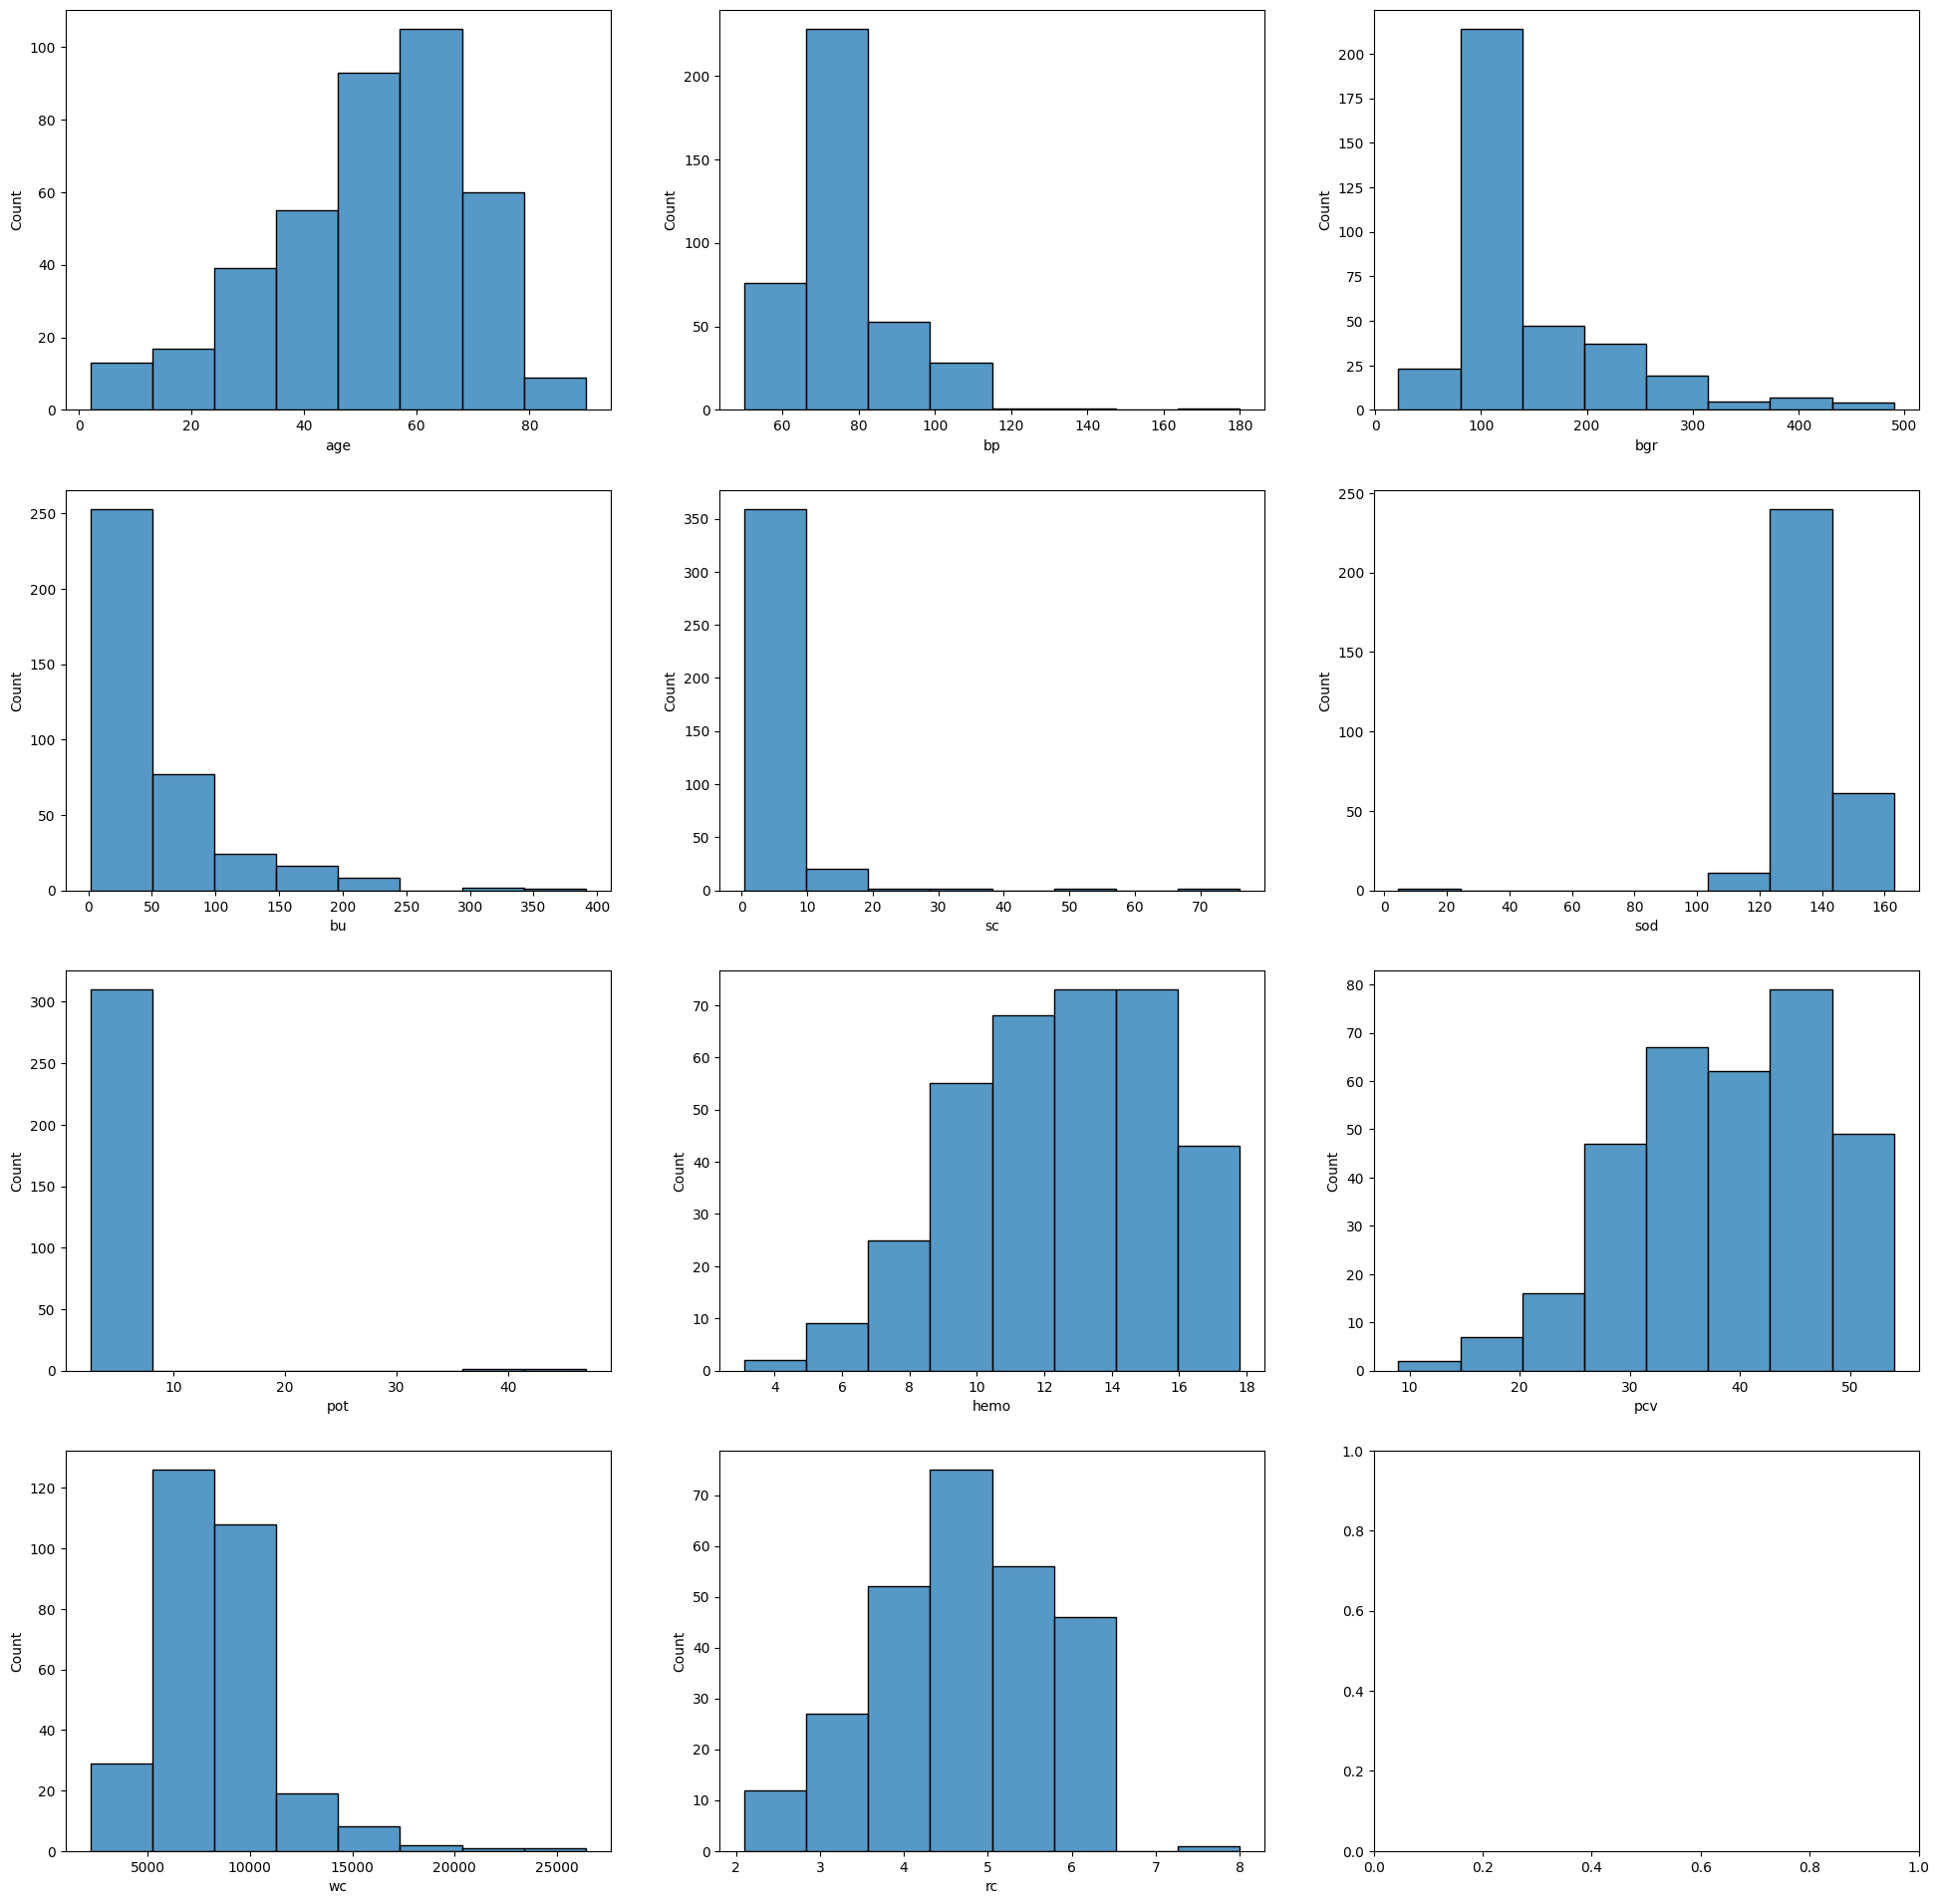
\includegraphics{Seebach_Lily_HW6_files/figure-pdf/cell-10-output-1.png}

Some variables are heavily skewed such as white blood cell count,
potassium, serum creatinine, blood urea, blood pressure, and blood
glucose random. Conversely, red blood cell count appears relatively
normally distribtued.

\begin{Shaded}
\begin{Highlighting}[]
\ImportTok{import}\NormalTok{ seaborn }\ImportTok{as}\NormalTok{ sns}
\ImportTok{import}\NormalTok{ matplotlib.pyplot }\ImportTok{as}\NormalTok{ plt}
\NormalTok{figure, axes }\OperatorTok{=}\NormalTok{ plt.subplots(}\DecValTok{7}\NormalTok{,}\DecValTok{2}\NormalTok{, sharex}\OperatorTok{=} \VariableTok{False}\NormalTok{, figsize}\OperatorTok{=}\NormalTok{(}\DecValTok{26}\NormalTok{,}\DecValTok{30}\NormalTok{))}
\NormalTok{k }\OperatorTok{=} \DecValTok{0}
\NormalTok{cat\_vars }\OperatorTok{=}\NormalTok{  data.select\_dtypes(include}\OperatorTok{=}\StringTok{\textquotesingle{}category\textquotesingle{}}\NormalTok{).columns}
\ControlFlowTok{for}\NormalTok{ i }\KeywordTok{in} \BuiltInTok{range}\NormalTok{(}\DecValTok{7}\NormalTok{):}
    \ControlFlowTok{for}\NormalTok{ j }\KeywordTok{in} \BuiltInTok{range}\NormalTok{(}\DecValTok{2}\NormalTok{):}
\NormalTok{        sns.countplot(ax }\OperatorTok{=}\NormalTok{ axes[i,j], data}\OperatorTok{=}\NormalTok{data, x }\OperatorTok{=} \BuiltInTok{str}\NormalTok{(cat\_vars[k]))}
\NormalTok{        k }\OperatorTok{=}\NormalTok{ k}\OperatorTok{+}\DecValTok{1}
\NormalTok{plt.show()}
\end{Highlighting}
\end{Shaded}

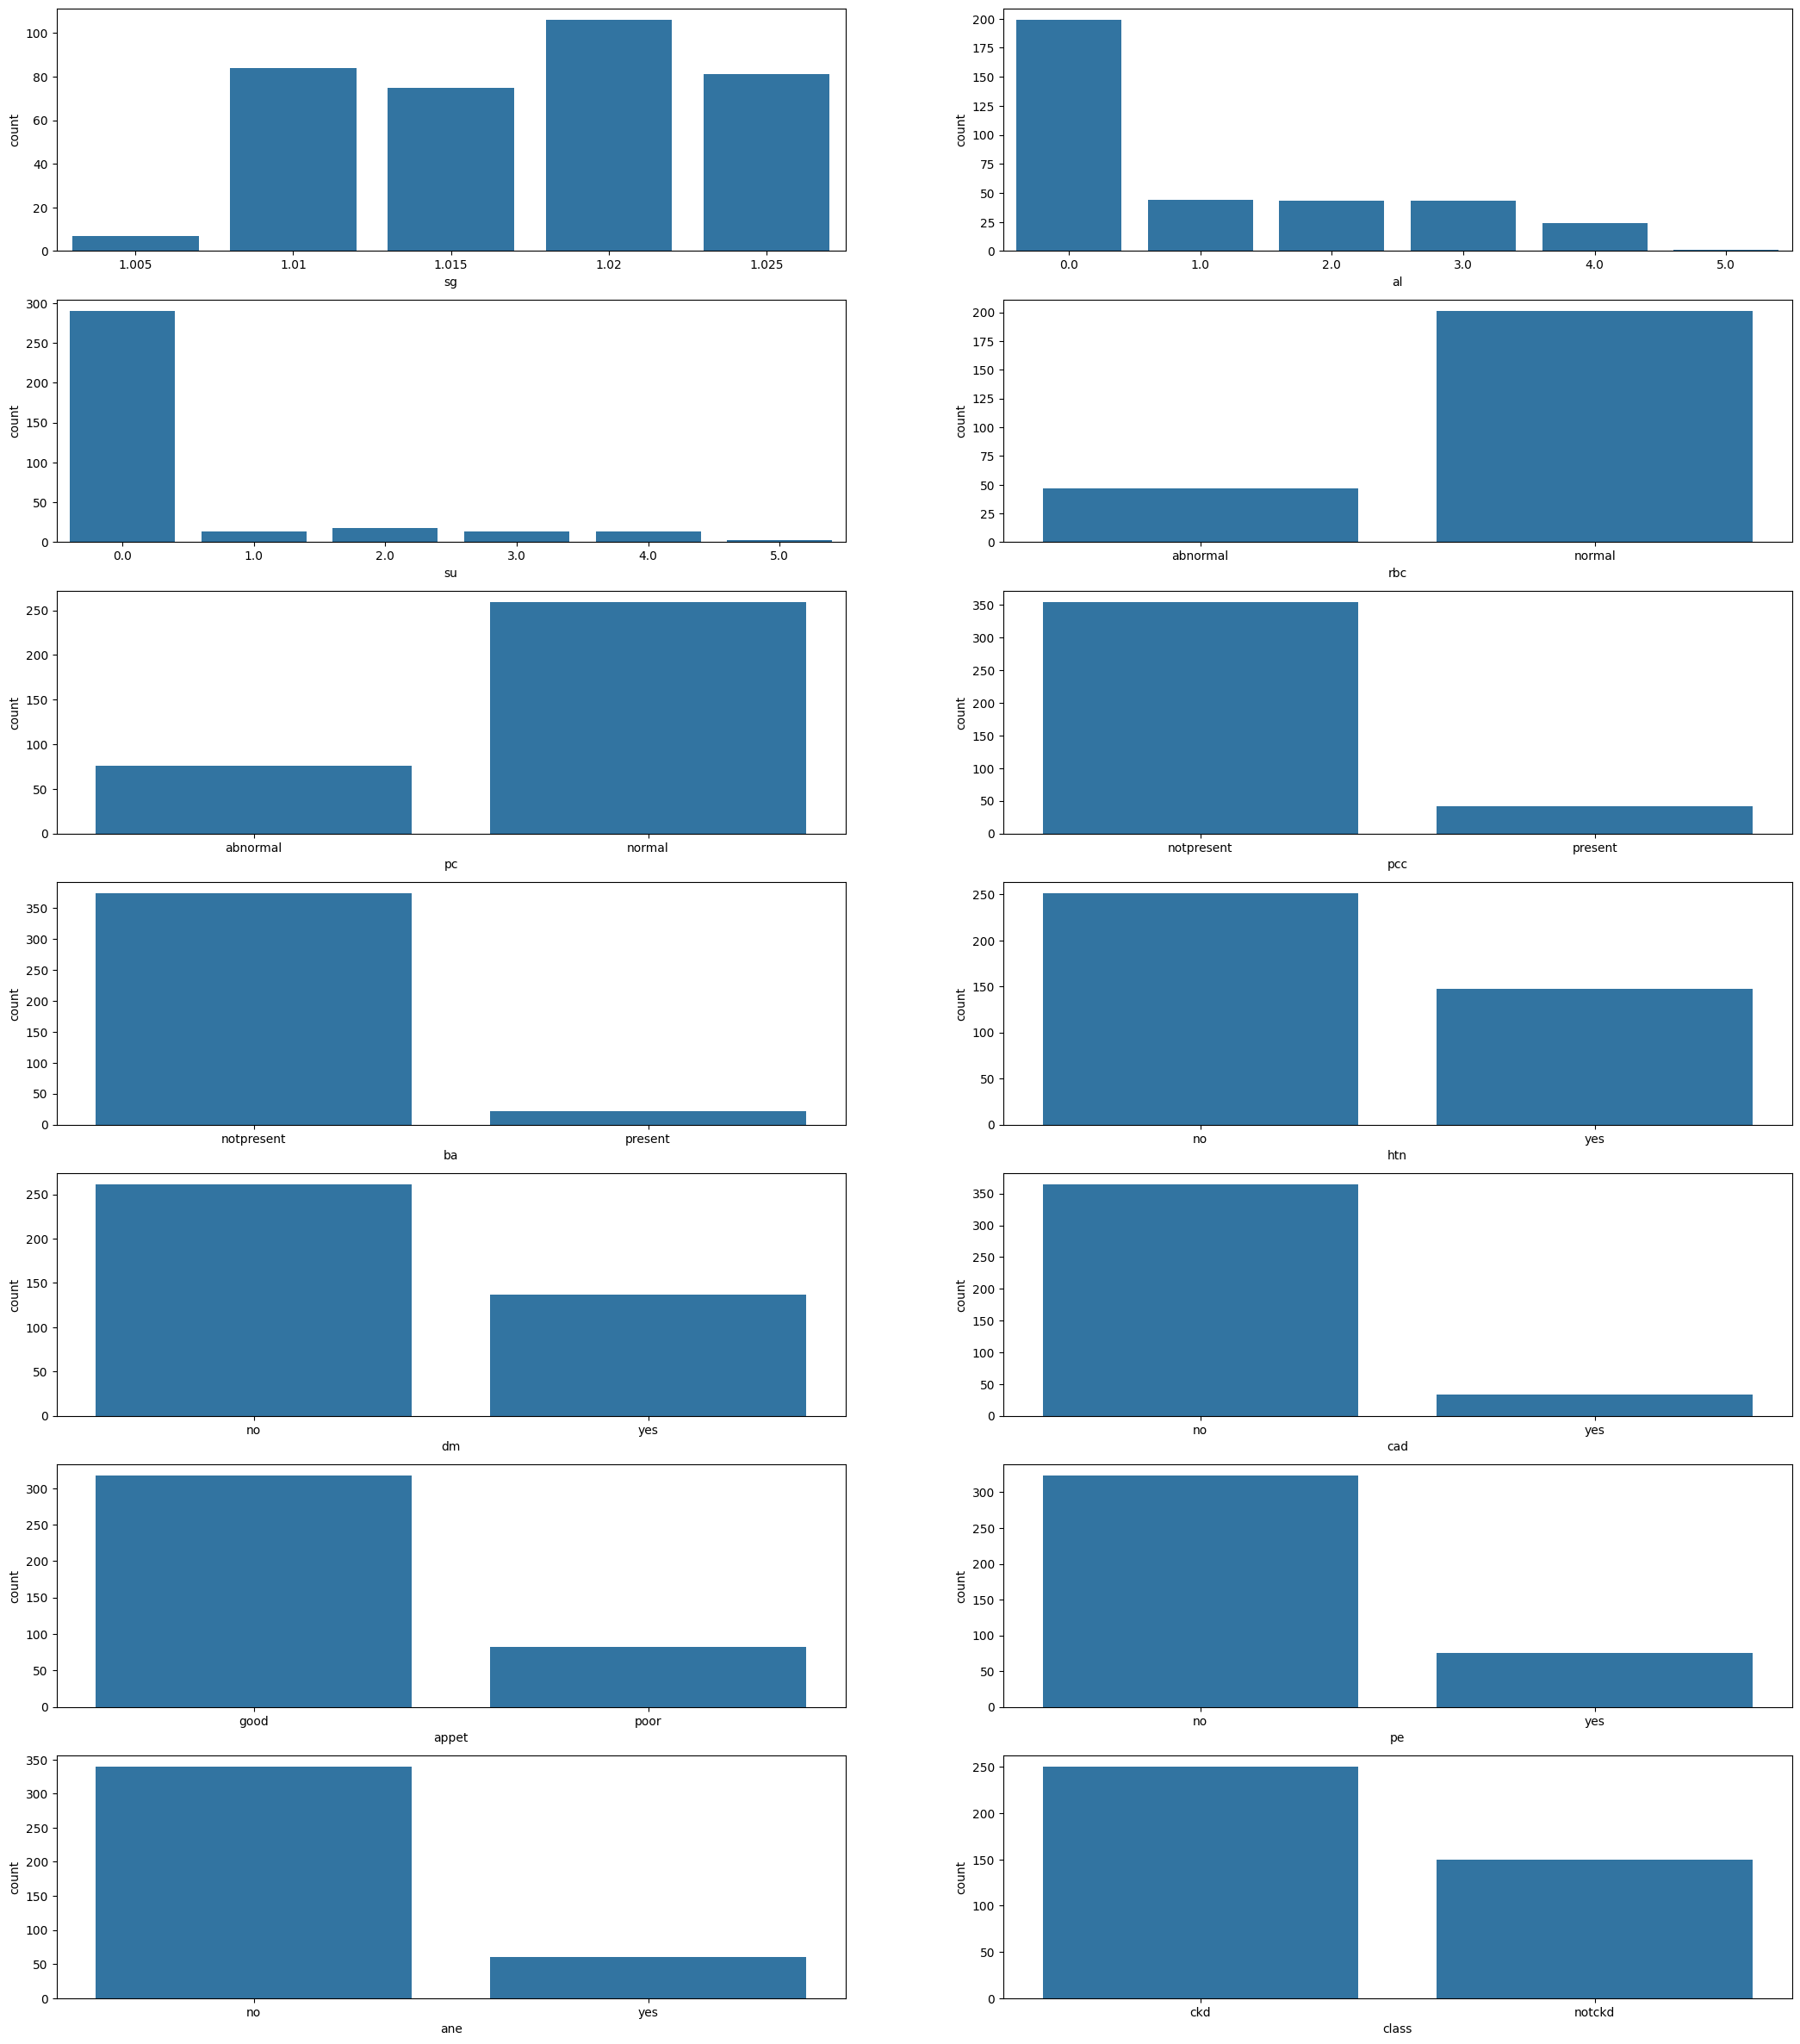
\includegraphics{Seebach_Lily_HW6_files/figure-pdf/cell-11-output-1.png}

We notice most categorical variables are heavily skewed. For example,
hypertension, diabetes mellitus, coronary artery disease, appetite,
pedal edema, and anemia all have many more instances of ``no'' than
``yes''. Red blood cells and pus cell display similar trends where by
``normal'' is more frequent than ``abnormal''. Pus cell clumps and
bacteria also display this trend where ``present'' is far less frequent
than ``not present''. It is important to note that class (ckd, notckd)
does not display this heavy skew. Although ``ckd'' is more frequent than
``notckd'', the two are relatively even.

\begin{enumerate}
\def\labelenumi{\arabic{enumi}.}
\setcounter{enumi}{3}
\tightlist
\item
  We now analyze variable relationships. We use a heatmap to check for
  correlation between numerical variables.
\end{enumerate}

\begin{Shaded}
\begin{Highlighting}[]
\NormalTok{num\_col }\OperatorTok{=}\NormalTok{ data.select\_dtypes(include }\OperatorTok{=} \StringTok{\textquotesingle{}float64\textquotesingle{}}\NormalTok{).columns}
\NormalTok{sns.heatmap(data[num\_col].corr(), annot}\OperatorTok{=}\VariableTok{True}\NormalTok{)}
\end{Highlighting}
\end{Shaded}

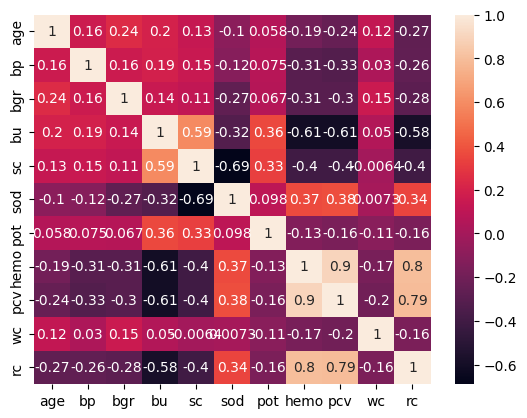
\includegraphics{Seebach_Lily_HW6_files/figure-pdf/cell-12-output-1.png}

From this heatmap we can see hemoglobin and packed cell volume,
hemoglobin and red blood cell count, and packed cell volume and red
blood cell count have a high positive correlation (\textgreater0.75).
Conversely, sodium and serum creatinine, hemoglobin and blood urea, and
packed cell volume and blood urea have a high negative correlation
(\textless-0.6). The least correlated variables are white blood cell
count and serum creatinine (0.0064). These correlations will likely
cause feature selection to drop one of the variables in highly
correlated variables.

\begin{enumerate}
\def\labelenumi{\arabic{enumi}.}
\setcounter{enumi}{4}
\tightlist
\item
  We remove observations with missing values in order to conduct
  subgroup analysis and for future use.
\end{enumerate}

\begin{Shaded}
\begin{Highlighting}[]
\NormalTok{data }\OperatorTok{=}\NormalTok{ data.dropna(ignore\_index}\OperatorTok{=}\VariableTok{True}\NormalTok{) }\CommentTok{\# drop observations with missing values}
\end{Highlighting}
\end{Shaded}

While this greatly reduces the data's sample size, it avoids adding bias
by entering other values for missing values (eg. mean, median, or mode),
or filling them in another way.

\begin{enumerate}
\def\labelenumi{\arabic{enumi}.}
\setcounter{enumi}{5}
\item
  We do not conduct outlier analysis. This is because outliers can be
  very important in diagnosing diseases in health data. By removing
  outliers, we would miss the opportunity to see how extreme values can
  help in finding disease risks.
\item
  We now conduct using K-means clustering on the data, after scaling and
  creating dummy variables, to conduct sub-group analysis.
\end{enumerate}

\begin{Shaded}
\begin{Highlighting}[]
\ImportTok{from}\NormalTok{ sklearn.cluster }\ImportTok{import}\NormalTok{ KMeans}
\ImportTok{from}\NormalTok{ sklearn.metrics }\ImportTok{import}\NormalTok{ silhouette\_samples, silhouette\_score}
\ImportTok{import}\NormalTok{ matplotlib.cm }\ImportTok{as}\NormalTok{ cm}
\ImportTok{from}\NormalTok{ sklearn.preprocessing }\ImportTok{import}\NormalTok{ scale}
\NormalTok{scaled\_data }\OperatorTok{=}\NormalTok{ data.copy()}
\NormalTok{scaled\_data[num\_col] }\OperatorTok{=}\NormalTok{ pd.DataFrame(scale(data[num\_col]))}
\NormalTok{dummy }\OperatorTok{=}\NormalTok{ pd.get\_dummies(data }\OperatorTok{=}\NormalTok{ scaled\_data, columns }\OperatorTok{=}\NormalTok{ cat\_vars)}
\NormalTok{scaled\_data }\OperatorTok{=}\NormalTok{ scaled\_data.drop(cat\_vars, axis }\OperatorTok{=} \DecValTok{1}\NormalTok{)}
\NormalTok{scaled\_data }\OperatorTok{=}\NormalTok{ pd.concat([scaled\_data, dummy], axis }\OperatorTok{=} \DecValTok{1}\NormalTok{)}
\NormalTok{scaled\_data }\OperatorTok{=}\NormalTok{ scaled\_data.drop([}\StringTok{\textquotesingle{}class\_ckd\textquotesingle{}}\NormalTok{,}\StringTok{\textquotesingle{}class\_notckd\textquotesingle{}}\NormalTok{], axis }\OperatorTok{=} \DecValTok{1}\NormalTok{)}
\NormalTok{range\_n\_clusters }\OperatorTok{=}\NormalTok{ [}\DecValTok{2}\NormalTok{, }\DecValTok{3}\NormalTok{]}
\ControlFlowTok{for}\NormalTok{ n\_clusters }\KeywordTok{in}\NormalTok{ range\_n\_clusters:}
\NormalTok{    km }\OperatorTok{=}\NormalTok{ KMeans(n\_clusters }\OperatorTok{=}\NormalTok{ n\_clusters, n\_init }\OperatorTok{=} \DecValTok{20}\NormalTok{, random\_state}\OperatorTok{=}\DecValTok{0}\NormalTok{)}
\NormalTok{    cluster\_labels\_km }\OperatorTok{=}\NormalTok{ km.fit\_predict(scaled\_data)}
    \CommentTok{\# average silhouette score}
\NormalTok{    silhouette\_avg\_km }\OperatorTok{=}\NormalTok{ silhouette\_score(scaled\_data, cluster\_labels\_km)}
    \CommentTok{\# compute the silhouette scores for each sample}
\NormalTok{    sample\_silhouette\_values }\OperatorTok{=}\NormalTok{ silhouette\_samples(scaled\_data, cluster\_labels\_km)}
\NormalTok{    fig, ax1 }\OperatorTok{=}\NormalTok{ plt.subplots(}\DecValTok{1}\NormalTok{, }\DecValTok{1}\NormalTok{)}
\NormalTok{    fig.set\_size\_inches(}\DecValTok{18}\NormalTok{, }\DecValTok{7}\NormalTok{)}
\NormalTok{    ax1.set\_xlim([}\OperatorTok{{-}}\FloatTok{0.3}\NormalTok{, }\DecValTok{1}\NormalTok{])}\CommentTok{\# change this based on the silhouette range}
\NormalTok{    y\_lower }\OperatorTok{=} \DecValTok{10}
    \ControlFlowTok{for}\NormalTok{ i }\KeywordTok{in} \BuiltInTok{range}\NormalTok{(n\_clusters):}
        \CommentTok{\# Aggregate the silhouette scores for samples belonging to}
        \CommentTok{\# cluster i, and sort them}
\NormalTok{        ith\_cluster\_silhouette\_values }\OperatorTok{=}\NormalTok{ sample\_silhouette\_values[cluster\_labels\_km }\OperatorTok{==}\NormalTok{ i]}
\NormalTok{        ith\_cluster\_silhouette\_values.sort()}
\NormalTok{        size\_cluster\_i }\OperatorTok{=}\NormalTok{ ith\_cluster\_silhouette\_values.shape[}\DecValTok{0}\NormalTok{]}
\NormalTok{        y\_upper }\OperatorTok{=}\NormalTok{ y\_lower }\OperatorTok{+}\NormalTok{ size\_cluster\_i}
\NormalTok{        color }\OperatorTok{=}\NormalTok{ cm.nipy\_spectral(}\BuiltInTok{float}\NormalTok{(i) }\OperatorTok{/}\NormalTok{ n\_clusters)}
\NormalTok{        ax1.fill\_betweenx(}
\NormalTok{            y}\OperatorTok{=}\NormalTok{np.arange(y\_lower, y\_upper),}
\NormalTok{            x1}\OperatorTok{=}\DecValTok{0}\NormalTok{,}
\NormalTok{            x2}\OperatorTok{=}\NormalTok{ith\_cluster\_silhouette\_values,}
\NormalTok{            facecolor}\OperatorTok{=}\NormalTok{color,}
\NormalTok{            edgecolor}\OperatorTok{=}\NormalTok{color,}
\NormalTok{            alpha}\OperatorTok{=}\FloatTok{0.7}\NormalTok{,}
\NormalTok{        )}
        \CommentTok{\# label the silhouette plots with their cluster numbers at the middle}
\NormalTok{        ax1.text(}\OperatorTok{{-}}\FloatTok{0.05}\NormalTok{, y\_lower }\OperatorTok{+} \FloatTok{0.5} \OperatorTok{*}\NormalTok{ size\_cluster\_i, }\BuiltInTok{str}\NormalTok{(i))}
        \CommentTok{\# Compute the new y\_lower for next cluster silhouette scores}
\NormalTok{        y\_lower }\OperatorTok{=}\NormalTok{ y\_upper }\OperatorTok{+} \DecValTok{10}  
\NormalTok{    ax1.set\_title(}\StringTok{"The silhouette plot for various cluster"}\NormalTok{)}
\NormalTok{    ax1.set\_xlabel(}\StringTok{"The silhouette coefficient values"}\NormalTok{)}
\NormalTok{    ax1.set\_ylabel(}\StringTok{"Cluster label"}\NormalTok{)}
    \CommentTok{\# vertical line for average silhouette score of all the values}
\NormalTok{    ax1.axvline(x}\OperatorTok{=}\NormalTok{silhouette\_avg\_km, color}\OperatorTok{=}\StringTok{"red"}\NormalTok{, linestyle}\OperatorTok{=}\StringTok{"{-}{-}"}\NormalTok{)}
\NormalTok{    plt.title(}
        \StringTok{"Silhouette analysis for KMeans clustering on sample data with n\_clusters = }\SpecialCharTok{\%d}\StringTok{"}
        \OperatorTok{\%}\NormalTok{ n\_clusters,}
\NormalTok{        fontsize}\OperatorTok{=}\DecValTok{14}\NormalTok{,}
\NormalTok{        fontweight}\OperatorTok{=}\StringTok{"bold"}\NormalTok{,}
\NormalTok{    )}
\NormalTok{plt.show()}
\end{Highlighting}
\end{Shaded}

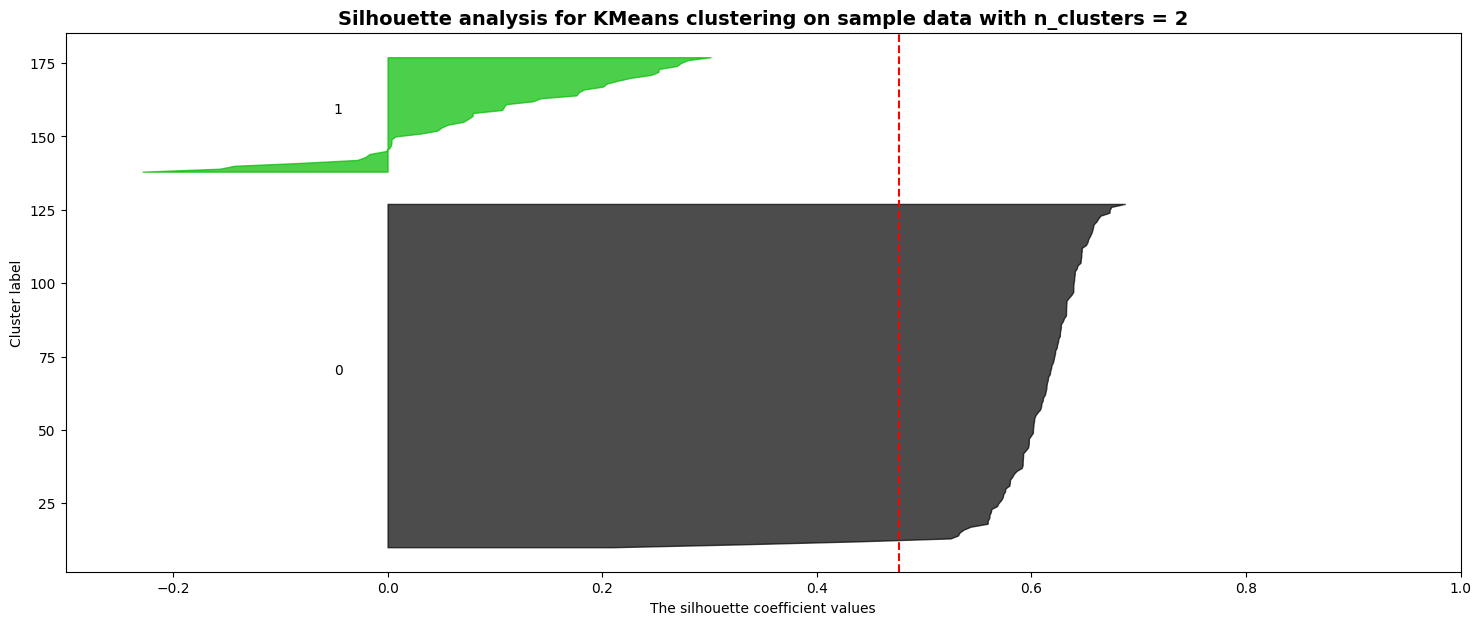
\includegraphics{Seebach_Lily_HW6_files/figure-pdf/cell-14-output-1.png}

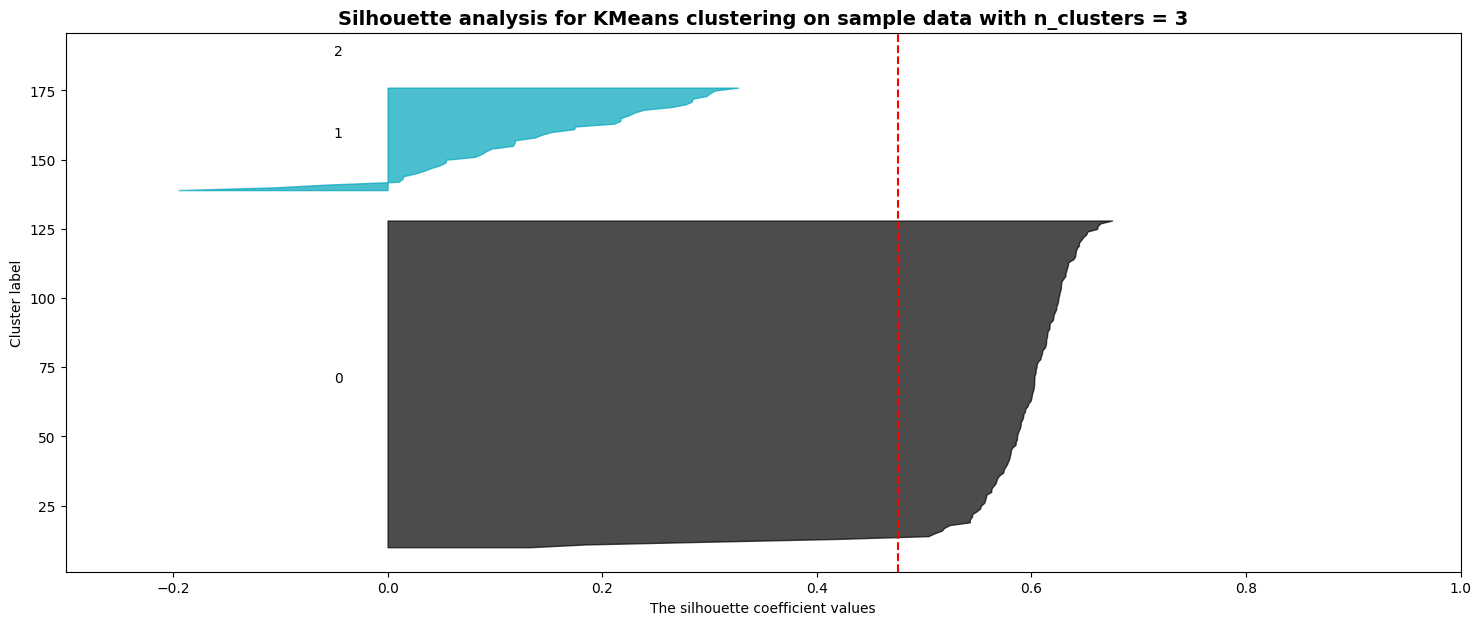
\includegraphics{Seebach_Lily_HW6_files/figure-pdf/cell-14-output-2.png}

There appears to be two subgroups, we now visualize them using PCA with
two PCs.

\begin{Shaded}
\begin{Highlighting}[]
\NormalTok{km1 }\OperatorTok{=}\NormalTok{ KMeans(n\_clusters}\OperatorTok{=}\DecValTok{2}\NormalTok{, n\_init}\OperatorTok{=}\DecValTok{20}\NormalTok{, random\_state}\OperatorTok{=}\DecValTok{0}\NormalTok{)}
\NormalTok{km1.fit(scaled\_data)}
\NormalTok{cluster\_labels\_km1 }\OperatorTok{=}\NormalTok{ km1.fit\_predict(scaled\_data)}
\ImportTok{from}\NormalTok{ sklearn.decomposition }\ImportTok{import}\NormalTok{ PCA, TruncatedSVD, FactorAnalysis}
\NormalTok{pca }\OperatorTok{=}\NormalTok{ PCA()}
\NormalTok{pc\_scores }\OperatorTok{=}\NormalTok{ pd.DataFrame(pca.fit\_transform(scaled\_data), index}\OperatorTok{=}\NormalTok{scaled\_data.index)}
\NormalTok{color\_idx }\OperatorTok{=}\NormalTok{ pd.factorize(cluster\_labels\_km1)[}\DecValTok{0}\NormalTok{]}
\NormalTok{cmap }\OperatorTok{=}\NormalTok{ plt.cm.jet}
\NormalTok{scatter }\OperatorTok{=}\NormalTok{ plt.scatter(pc\_scores.iloc[:,}\DecValTok{0}\NormalTok{], pc\_scores.iloc[:,}\DecValTok{1}\NormalTok{], c}\OperatorTok{=}\NormalTok{color\_idx, cmap}\OperatorTok{=}\NormalTok{cmap, alpha}\OperatorTok{=}\FloatTok{0.5}\NormalTok{, s}\OperatorTok{=}\DecValTok{50}\NormalTok{)}
\NormalTok{plt.ylabel(}\StringTok{\textquotesingle{}Principal Component 2\textquotesingle{}}\NormalTok{)}
\NormalTok{plt.xlabel(}\StringTok{\textquotesingle{}Principal Component 1\textquotesingle{}}\NormalTok{)}
\NormalTok{plt.show()}
\end{Highlighting}
\end{Shaded}

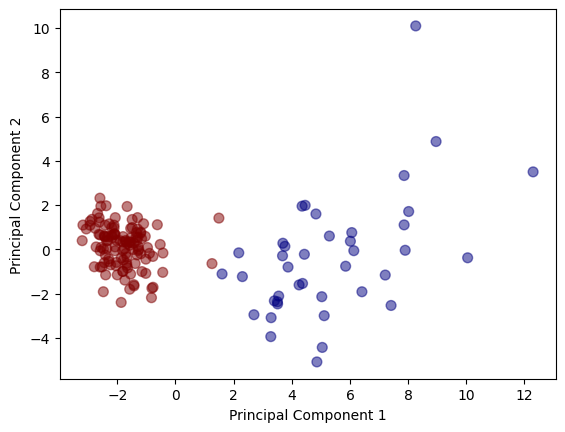
\includegraphics{Seebach_Lily_HW6_files/figure-pdf/cell-15-output-1.png}

From this analysis, we can see there is a clearly defined sub-group in
the bottom left corner based on the data.

\begin{enumerate}
\def\labelenumi{\arabic{enumi}.}
\setcounter{enumi}{7}
\tightlist
\item
  We now split the unscaled, original data into a 70/30 training/test
  split for testing, using a random seed of 1 and stratified sampling.
\end{enumerate}

\begin{Shaded}
\begin{Highlighting}[]
\ImportTok{from}\NormalTok{ sklearn.model\_selection }\ImportTok{import}\NormalTok{ train\_test\_split}
\NormalTok{y }\OperatorTok{=}\NormalTok{ data[}\StringTok{\textquotesingle{}class\textquotesingle{}}\NormalTok{]}
\NormalTok{x }\OperatorTok{=}\NormalTok{ data.drop(}\StringTok{\textquotesingle{}class\textquotesingle{}}\NormalTok{, axis }\OperatorTok{=} \DecValTok{1}\NormalTok{)}
\NormalTok{X\_train, X\_test, y\_train, y\_test }\OperatorTok{=}\NormalTok{ train\_test\_split(}
\NormalTok{x, y, test\_size}\OperatorTok{=}\FloatTok{0.3}\NormalTok{, random\_state}\OperatorTok{=}\DecValTok{1}\NormalTok{, stratify}\OperatorTok{=}\NormalTok{y)}
\end{Highlighting}
\end{Shaded}

\begin{enumerate}
\def\labelenumi{\arabic{enumi}.}
\setcounter{enumi}{8}
\item
  We choose two classifiers to address the classification problem. First
  we use k-nearest neighbours (KNN) then we use a decision tree. We
  choose these classifiers as they are supervised learning methods and
  decision trees are interpretable. Also, classic k-nearest neighbours
  is used for numerical variables only while decision trees can handle
  mixed variable types, allowing us to see how including categorical
  variables can affect performance.
\item
  We will use accuracy and sensitivity to compare the performance of the
  classifiers. Accuracy compares the overall performance while
  sensitivity will compare how good the classifier is at correctly
  identifying an individual with chronic kidney disease.
\item
  We use lasso regression to determine important features for KNN while
  decision trees automatically perform feature selection. We use the
  previous data which was scaled and uses dummy variables and select the
  corresponding testing and training values.
\end{enumerate}

\begin{Shaded}
\begin{Highlighting}[]
\ImportTok{from}\NormalTok{ sklearn.linear\_model }\ImportTok{import}\NormalTok{ Ridge, Lasso, ElasticNet, RidgeCV, LassoCV, ElasticNetCV}
\NormalTok{x\_train\_num }\OperatorTok{=}\NormalTok{ scaled\_data.iloc[X\_train.index]}
\NormalTok{y\_train\_num }\OperatorTok{=}\NormalTok{ y\_train.cat.codes}
\NormalTok{x\_test\_num }\OperatorTok{=}\NormalTok{ scaled\_data.iloc[X\_test.index]}
\NormalTok{lasso\_cv }\OperatorTok{=}\NormalTok{ LassoCV(alphas}\OperatorTok{=}\NormalTok{np.logspace(}\OperatorTok{{-}}\DecValTok{4}\NormalTok{, }\DecValTok{4}\NormalTok{, }\DecValTok{100}\NormalTok{), cv}\OperatorTok{=}\DecValTok{5}\NormalTok{, max\_iter}\OperatorTok{=}\DecValTok{1500}\NormalTok{)}
\NormalTok{lasso\_cv.fit(x\_train\_num, y\_train\_num)}
\NormalTok{m\_lasso }\OperatorTok{=}\NormalTok{ Lasso(alpha}\OperatorTok{=}\NormalTok{lasso\_cv.alpha\_)}
\NormalTok{m\_lasso.fit(x\_train\_num, y\_train\_num) }
\NormalTok{m\_lasso\_pre }\OperatorTok{=}\NormalTok{ m\_lasso.predict(x\_test\_num)}
\NormalTok{pd.DataFrame(\{}\StringTok{\textquotesingle{}Feature\textquotesingle{}}\NormalTok{: x\_train\_num.columns, }\StringTok{\textquotesingle{}Coefficient\textquotesingle{}}\NormalTok{: m\_lasso.coef\_.reshape(}\BuiltInTok{len}\NormalTok{(x\_train\_num.columns))\})}
\end{Highlighting}
\end{Shaded}

\begin{longtable}[]{@{}lll@{}}
\toprule\noalign{}
& Feature & Coefficient \\
\midrule\noalign{}
\endhead
\bottomrule\noalign{}
\endlastfoot
0 & age & -0.000000 \\
1 & bp & -0.000000 \\
2 & bgr & -0.000000 \\
3 & bu & -0.000000 \\
4 & sc & -0.000000 \\
5 & sod & 0.000000 \\
6 & pot & -0.000000 \\
7 & hemo & 0.000000 \\
8 & pcv & 0.000000 \\
9 & wc & -0.000000 \\
10 & rc & 0.000000 \\
11 & age & -0.000000 \\
12 & bp & -0.000000 \\
13 & bgr & -0.000092 \\
14 & bu & -0.000000 \\
15 & sc & -0.000000 \\
16 & sod & 0.000101 \\
17 & pot & -0.000000 \\
18 & hemo & 0.000135 \\
19 & pcv & 0.000262 \\
20 & wc & -0.000062 \\
21 & rc & 0.000000 \\
22 & sg\_1.005 & 0.000000 \\
23 & sg\_1.01 & -0.000000 \\
24 & sg\_1.015 & -0.000000 \\
25 & sg\_1.02 & 0.000000 \\
26 & sg\_1.025 & 0.000000 \\
27 & al\_0.0 & 0.998354 \\
28 & al\_1.0 & -0.000000 \\
29 & al\_2.0 & -0.000000 \\
30 & al\_3.0 & -0.000000 \\
31 & al\_4.0 & -0.000000 \\
32 & al\_5.0 & 0.000000 \\
33 & su\_0.0 & 0.000000 \\
34 & su\_1.0 & -0.000000 \\
35 & su\_2.0 & -0.000000 \\
36 & su\_3.0 & -0.000000 \\
37 & su\_4.0 & -0.000000 \\
38 & su\_5.0 & -0.000000 \\
39 & rbc\_abnormal & -0.000000 \\
40 & rbc\_normal & 0.000000 \\
41 & pc\_abnormal & -0.000000 \\
42 & pc\_normal & 0.000000 \\
43 & pcc\_notpresent & 0.000000 \\
44 & pcc\_present & -0.000000 \\
45 & ba\_notpresent & 0.000000 \\
46 & ba\_present & -0.000000 \\
47 & htn\_no & 0.000000 \\
48 & htn\_yes & -0.000000 \\
49 & dm\_no & 0.000000 \\
50 & dm\_yes & -0.000000 \\
51 & cad\_no & 0.000000 \\
52 & cad\_yes & -0.000000 \\
53 & appet\_good & 0.000000 \\
54 & appet\_poor & -0.000000 \\
55 & pe\_no & 0.000000 \\
56 & pe\_yes & -0.000000 \\
57 & ane\_no & 0.000000 \\
58 & ane\_yes & -0.000000 \\
\end{longtable}

Using lasso regression, we see that many variables have been given a
coefficient of zero. Specifically all coefficients have been shrunk to
zero except blood glucose random, sodium, hemoglobin, packed cell
volume, white blood cell count, and albumin. Note that albumin received
by far the largest coefficient.

\begin{enumerate}
\def\labelenumi{\arabic{enumi}.}
\setcounter{enumi}{11}
\tightlist
\item
  We now implement 5-fold cross validation for KNN with the scaled
  numerical variables not given a coefficient of 0 in the lasso
  regression process, and decision tree with all the variables. First we
  petform the cross-validation using the test set to select the best
  value of k.
\end{enumerate}

\begin{Shaded}
\begin{Highlighting}[]
\CommentTok{\#\# KNN Implementation}
\ImportTok{from}\NormalTok{ sklearn.model\_selection }\ImportTok{import}\NormalTok{ cross\_val\_score}
\NormalTok{X\_train\_red }\OperatorTok{=}\NormalTok{ X\_train.drop([}\StringTok{\textquotesingle{}age\textquotesingle{}}\NormalTok{, }\StringTok{\textquotesingle{}bp\textquotesingle{}}\NormalTok{, }\StringTok{\textquotesingle{}sg\textquotesingle{}}\NormalTok{,}\StringTok{\textquotesingle{}al\textquotesingle{}}\NormalTok{,}\StringTok{\textquotesingle{}su\textquotesingle{}}\NormalTok{,}\StringTok{\textquotesingle{}rbc\textquotesingle{}}\NormalTok{,}\StringTok{\textquotesingle{}pc\textquotesingle{}}\NormalTok{,}\StringTok{\textquotesingle{}pcc\textquotesingle{}}\NormalTok{,}\StringTok{\textquotesingle{}ba\textquotesingle{}}\NormalTok{,}\StringTok{\textquotesingle{}bu\textquotesingle{}}\NormalTok{,}\StringTok{\textquotesingle{}sc\textquotesingle{}}\NormalTok{,}\StringTok{\textquotesingle{}pot\textquotesingle{}}\NormalTok{,}\StringTok{\textquotesingle{}rc\textquotesingle{}}\NormalTok{,}\StringTok{\textquotesingle{}htn\textquotesingle{}}\NormalTok{,}\StringTok{\textquotesingle{}dm\textquotesingle{}}\NormalTok{,}\StringTok{\textquotesingle{}cad\textquotesingle{}}\NormalTok{,}\StringTok{\textquotesingle{}appet\textquotesingle{}}\NormalTok{,}\StringTok{\textquotesingle{}pe\textquotesingle{}}\NormalTok{,}\StringTok{\textquotesingle{}ane\textquotesingle{}}\NormalTok{], axis}\OperatorTok{=}\DecValTok{1}\NormalTok{)}
\NormalTok{X\_test\_red }\OperatorTok{=}\NormalTok{  X\_test.drop([}\StringTok{\textquotesingle{}age\textquotesingle{}}\NormalTok{, }\StringTok{\textquotesingle{}bp\textquotesingle{}}\NormalTok{, }\StringTok{\textquotesingle{}sg\textquotesingle{}}\NormalTok{,}\StringTok{\textquotesingle{}al\textquotesingle{}}\NormalTok{,}\StringTok{\textquotesingle{}su\textquotesingle{}}\NormalTok{,}\StringTok{\textquotesingle{}rbc\textquotesingle{}}\NormalTok{,}\StringTok{\textquotesingle{}pc\textquotesingle{}}\NormalTok{,}\StringTok{\textquotesingle{}pcc\textquotesingle{}}\NormalTok{,}\StringTok{\textquotesingle{}ba\textquotesingle{}}\NormalTok{,}\StringTok{\textquotesingle{}bu\textquotesingle{}}\NormalTok{,}\StringTok{\textquotesingle{}sc\textquotesingle{}}\NormalTok{,}\StringTok{\textquotesingle{}pot\textquotesingle{}}\NormalTok{,}\StringTok{\textquotesingle{}rc\textquotesingle{}}\NormalTok{,}\StringTok{\textquotesingle{}htn\textquotesingle{}}\NormalTok{,}\StringTok{\textquotesingle{}dm\textquotesingle{}}\NormalTok{,}\StringTok{\textquotesingle{}cad\textquotesingle{}}\NormalTok{,}\StringTok{\textquotesingle{}appet\textquotesingle{}}\NormalTok{,}\StringTok{\textquotesingle{}pe\textquotesingle{}}\NormalTok{,}\StringTok{\textquotesingle{}ane\textquotesingle{}}\NormalTok{], axis}\OperatorTok{=}\DecValTok{1}\NormalTok{)}
\NormalTok{X\_test\_red }\OperatorTok{=}\NormalTok{ scale(X\_test\_red)}
\NormalTok{X\_train\_red }\OperatorTok{=}\NormalTok{ scale(X\_train\_red)}

\ImportTok{from}\NormalTok{ sklearn }\ImportTok{import}\NormalTok{ neighbors}
\ImportTok{from}\NormalTok{ sklearn }\ImportTok{import}\NormalTok{ metrics}
\NormalTok{k\_range }\OperatorTok{=} \BuiltInTok{range}\NormalTok{(}\DecValTok{1}\NormalTok{, }\DecValTok{6}\NormalTok{)}
\NormalTok{cv\_scores }\OperatorTok{=}\NormalTok{ [] }
\ControlFlowTok{for}\NormalTok{ k }\KeywordTok{in}\NormalTok{ k\_range:}
\NormalTok{    knn\_cv }\OperatorTok{=}\NormalTok{ neighbors.KNeighborsClassifier(n\_neighbors}\OperatorTok{=}\NormalTok{k)}
\NormalTok{    cv\_scores\_k }\OperatorTok{=}\NormalTok{ cross\_val\_score(knn\_cv, X\_train\_red, y\_train, cv}\OperatorTok{=}\DecValTok{5}\NormalTok{)}
\NormalTok{    cv\_scores.append(np.mean(cv\_scores\_k))}
\NormalTok{plt.plot(k\_range, cv\_scores)}
\NormalTok{plt.xlabel(}\StringTok{\textquotesingle{}K\textquotesingle{}}\NormalTok{)}
\NormalTok{plt.ylabel(}\StringTok{\textquotesingle{}5{-}fold CV accuracy\textquotesingle{}}\NormalTok{)}
\NormalTok{plt.xticks(}\BuiltInTok{range}\NormalTok{(}\DecValTok{1}\NormalTok{,}\DecValTok{6}\NormalTok{))}
\NormalTok{plt.show()}
\end{Highlighting}
\end{Shaded}

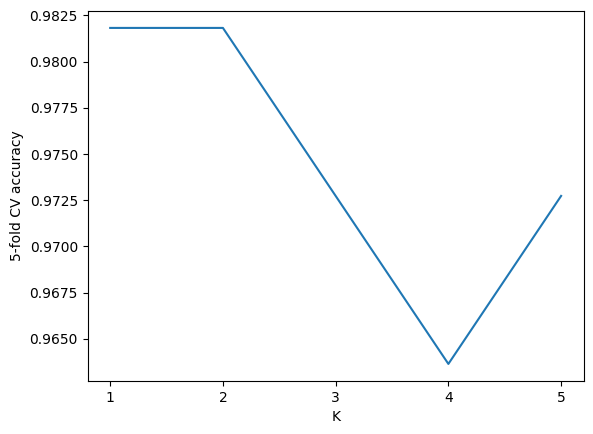
\includegraphics{Seebach_Lily_HW6_files/figure-pdf/cell-18-output-1.png}

Selecting K = 2 to maximize accuracy and minimize variance:

\begin{Shaded}
\begin{Highlighting}[]
\NormalTok{knn }\OperatorTok{=}\NormalTok{ neighbors.KNeighborsClassifier(n\_neighbors }\OperatorTok{=} \DecValTok{2}\NormalTok{)}
\NormalTok{knn.fit(X\_train\_red,y\_train)}
\NormalTok{pred }\OperatorTok{=}\NormalTok{ knn.predict(X\_test\_red)}
\ImportTok{from}\NormalTok{ sklearn.metrics }\ImportTok{import}\NormalTok{ mean\_squared\_error, confusion\_matrix, classification\_report}
\NormalTok{cm }\OperatorTok{=}\NormalTok{ pd.DataFrame(confusion\_matrix(y\_test, pred), index}\OperatorTok{=}\NormalTok{[}\StringTok{\textquotesingle{}No CKD\textquotesingle{}}\NormalTok{, }\StringTok{\textquotesingle{}CKD\textquotesingle{}}\NormalTok{], columns}\OperatorTok{=}\NormalTok{[}\StringTok{\textquotesingle{}No CKD\textquotesingle{}}\NormalTok{, }\StringTok{\textquotesingle{}CKD\textquotesingle{}}\NormalTok{])}
\NormalTok{sensitivity }\OperatorTok{=}\NormalTok{ cm.iloc[}\DecValTok{1}\NormalTok{,}\DecValTok{1}\NormalTok{]}\OperatorTok{/}\NormalTok{(cm.iloc[}\DecValTok{1}\NormalTok{,}\DecValTok{0}\NormalTok{]}\OperatorTok{+}\NormalTok{cm.iloc[}\DecValTok{1}\NormalTok{,}\DecValTok{1}\NormalTok{])}
\BuiltInTok{print}\NormalTok{(}\StringTok{\textquotesingle{}Sensitivity : \textquotesingle{}}\NormalTok{, sensitivity)}
\BuiltInTok{print}\NormalTok{(}\StringTok{\textquotesingle{}Accuracy : \textquotesingle{}}\NormalTok{, }\BuiltInTok{round}\NormalTok{(metrics.accuracy\_score(y\_test, pred),}\DecValTok{2}\NormalTok{))}
\end{Highlighting}
\end{Shaded}

\begin{verbatim}
Sensitivity :  0.9714285714285714
Accuracy :  0.98
\end{verbatim}

Now using a decision tree using the original data with dummy variables
for categorical variables (all variables, unscaled).

\begin{Shaded}
\begin{Highlighting}[]
\ImportTok{from}\NormalTok{ sklearn.tree }\ImportTok{import}\NormalTok{ DecisionTreeClassifier, DecisionTreeRegressor, plot\_tree}
\ControlFlowTok{for}\NormalTok{ col }\KeywordTok{in}\NormalTok{ cat\_vars.drop(}\StringTok{\textquotesingle{}class\textquotesingle{}}\NormalTok{):}
\NormalTok{    X\_train[col] }\OperatorTok{=}\NormalTok{ pd.Categorical(X\_train[col]).codes}
\NormalTok{    X\_test[col] }\OperatorTok{=}\NormalTok{ pd.Categorical(X\_test[col]).codes}
\NormalTok{cs\_dt }\OperatorTok{=}\NormalTok{ DecisionTreeClassifier(}
\NormalTok{    max\_depth }\OperatorTok{=} \DecValTok{15}\NormalTok{, }
\NormalTok{    random\_state}\OperatorTok{=}\DecValTok{1}
\NormalTok{) }
\NormalTok{cs\_dt.fit(X\_train, y\_train)}
\end{Highlighting}
\end{Shaded}

\begin{verbatim}
DecisionTreeClassifier(max_depth=15, random_state=1)
\end{verbatim}

\begin{Shaded}
\begin{Highlighting}[]
\CommentTok{\#\# Decision Tree}
\ImportTok{from}\NormalTok{ sklearn.tree }\ImportTok{import}\NormalTok{ DecisionTreeClassifier, DecisionTreeRegressor, plot\_tree}
\NormalTok{cs\_dt }\OperatorTok{=}\NormalTok{ DecisionTreeClassifier(}
\NormalTok{    max\_depth }\OperatorTok{=} \DecValTok{15}\NormalTok{,}
\NormalTok{    random\_state}\OperatorTok{=}\DecValTok{1}
\NormalTok{    ) }
\NormalTok{cs\_dt.fit(X\_train, y\_train)}
\NormalTok{fig, axes }\OperatorTok{=}\NormalTok{ plt.subplots(}
\NormalTok{    nrows }\OperatorTok{=} \DecValTok{1}\NormalTok{,ncols }\OperatorTok{=} \DecValTok{1}\NormalTok{,figsize }\OperatorTok{=}\NormalTok{ (}\DecValTok{4}\NormalTok{,}\DecValTok{4}\NormalTok{), dpi}\OperatorTok{=}\DecValTok{300}
\NormalTok{    )}
\NormalTok{plot\_tree(}
\NormalTok{    cs\_dt, }
\NormalTok{    max\_depth}\OperatorTok{=} \DecValTok{5}\NormalTok{, }
\NormalTok{    feature\_names }\OperatorTok{=}\NormalTok{ X\_train.columns.tolist(), }
\NormalTok{    class\_names}\OperatorTok{=}\NormalTok{[}\StringTok{\textquotesingle{}CKD\textquotesingle{}}\NormalTok{, }\StringTok{\textquotesingle{}No CKD\textquotesingle{}}\NormalTok{], }
\NormalTok{    filled }\OperatorTok{=} \VariableTok{True}
\NormalTok{    )}
\end{Highlighting}
\end{Shaded}

\begin{verbatim}
[Text(0.5, 0.75, 'al <= 0.5\ngini = 0.397\nsamples = 110\nvalue = [30.0, 80.0]\nclass = No CKD'),
 Text(0.25, 0.25, 'gini = 0.0\nsamples = 80\nvalue = [0, 80]\nclass = No CKD'),
 Text(0.75, 0.25, 'gini = 0.0\nsamples = 30\nvalue = [30, 0]\nclass = CKD')]
\end{verbatim}

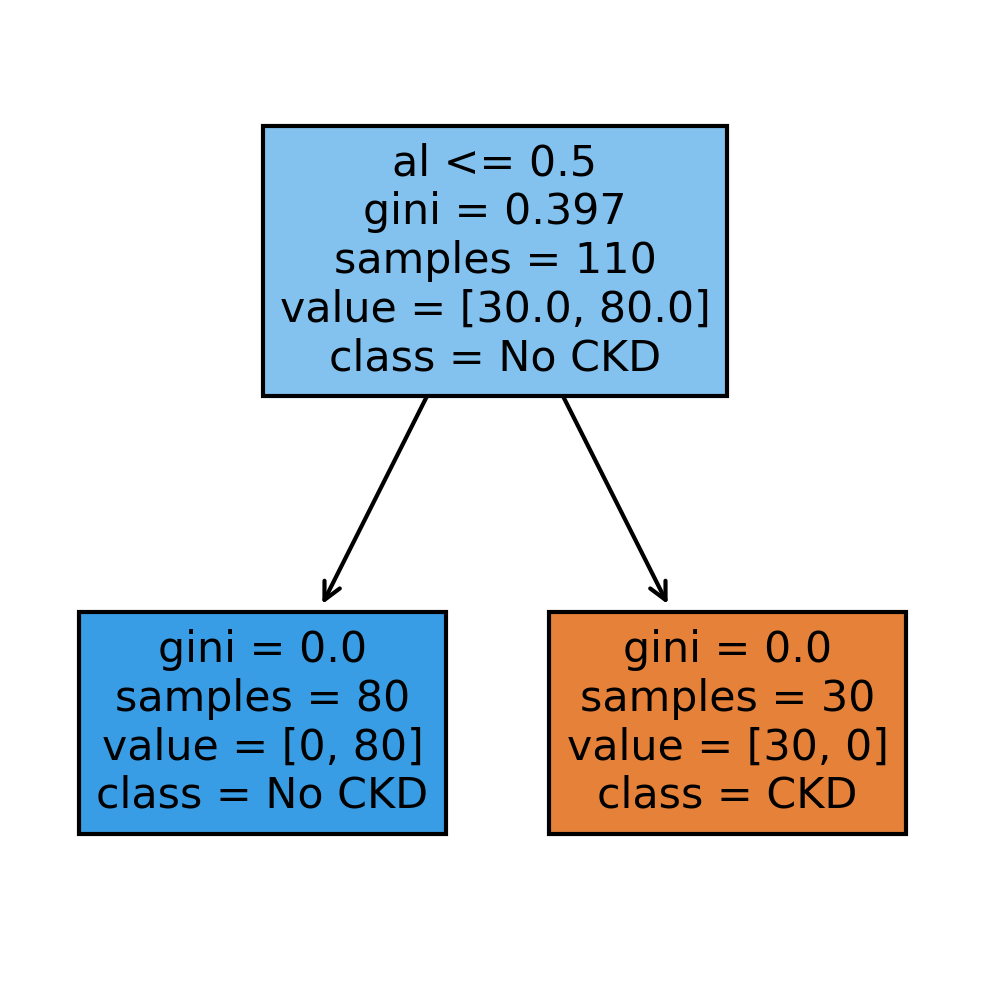
\includegraphics{Seebach_Lily_HW6_files/figure-pdf/cell-21-output-2.png}

Using a pruning tree to maximize accuaracy:

\begin{Shaded}
\begin{Highlighting}[]
\NormalTok{path }\OperatorTok{=}\NormalTok{ cs\_dt.cost\_complexity\_pruning\_path(}
\NormalTok{    x\_train\_num, }
\NormalTok{    y\_train}
\NormalTok{)}
\NormalTok{ccp\_alphas, impurities }\OperatorTok{=}\NormalTok{ path.ccp\_alphas, path.impurities}
\NormalTok{clfs }\OperatorTok{=}\NormalTok{ [] }\CommentTok{\# save fitted trees with different alphas}
\ControlFlowTok{for}\NormalTok{ ccp\_alpha }\KeywordTok{in}\NormalTok{ ccp\_alphas:}
\NormalTok{    clf }\OperatorTok{=}\NormalTok{ DecisionTreeClassifier(}
\NormalTok{        ccp\_alpha}\OperatorTok{=}\NormalTok{ccp\_alpha}
\NormalTok{        )}
\NormalTok{    clf.fit(x\_train\_num, y\_train)}
\NormalTok{    clfs.append(clf)}
\NormalTok{depth }\OperatorTok{=}\NormalTok{ [clf.tree\_.max\_depth }\ControlFlowTok{for}\NormalTok{ clf }\KeywordTok{in}\NormalTok{ clfs]}
\NormalTok{test\_score }\OperatorTok{=}\NormalTok{ [clf.score(x\_test\_num, y\_test) }\ControlFlowTok{for}\NormalTok{ clf }\KeywordTok{in}\NormalTok{ clfs]}
\NormalTok{plt.plot(depth, test\_score)}
\NormalTok{plt.xlabel(}\StringTok{\textquotesingle{}Depth\textquotesingle{}}\NormalTok{)}
\NormalTok{plt.ylabel(}\StringTok{\textquotesingle{}Accuracy\textquotesingle{}}\NormalTok{)}
\NormalTok{plt.show()}
\end{Highlighting}
\end{Shaded}

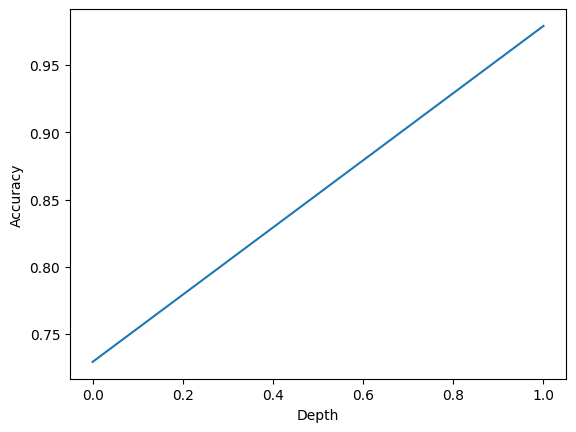
\includegraphics{Seebach_Lily_HW6_files/figure-pdf/cell-22-output-1.png}

Here, it appears the variable albumin is such a prominent variable in
detecting chronic kidney disease that no other variables are considered
in the process.

\begin{Shaded}
\begin{Highlighting}[]
\NormalTok{cs\_dt }\OperatorTok{=}\NormalTok{ DecisionTreeClassifier(}
\NormalTok{    max\_depth }\OperatorTok{=} \DecValTok{1}\NormalTok{,}
\NormalTok{    random\_state}\OperatorTok{=}\DecValTok{1}
\NormalTok{) }
\NormalTok{cs\_dt.fit(X\_train, y\_train)}
\NormalTok{pred }\OperatorTok{=}\NormalTok{ cs\_dt.predict(X\_test)}
\NormalTok{cm }\OperatorTok{=}\NormalTok{ pd.DataFrame(confusion\_matrix(y\_test, pred), index}\OperatorTok{=}\NormalTok{[}\StringTok{\textquotesingle{}No CKD\textquotesingle{}}\NormalTok{, }\StringTok{\textquotesingle{}CKD\textquotesingle{}}\NormalTok{], columns}\OperatorTok{=}\NormalTok{[}\StringTok{\textquotesingle{}No CKD\textquotesingle{}}\NormalTok{, }\StringTok{\textquotesingle{}CKD\textquotesingle{}}\NormalTok{])}
\NormalTok{cm.index.name }\OperatorTok{=} \StringTok{\textquotesingle{}True\textquotesingle{}}
\NormalTok{cm.columns.name }\OperatorTok{=} \StringTok{\textquotesingle{}Predicted\textquotesingle{}}
\NormalTok{sensitivity }\OperatorTok{=}\NormalTok{ cm.iloc[}\DecValTok{1}\NormalTok{,}\DecValTok{1}\NormalTok{]}\OperatorTok{/}\NormalTok{(cm.iloc[}\DecValTok{1}\NormalTok{,}\DecValTok{0}\NormalTok{]}\OperatorTok{+}\NormalTok{cm.iloc[}\DecValTok{1}\NormalTok{,}\DecValTok{1}\NormalTok{])}
\BuiltInTok{print}\NormalTok{(}\StringTok{\textquotesingle{}Sensitivity : \textquotesingle{}}\NormalTok{, sensitivity)}
\BuiltInTok{print}\NormalTok{(}\StringTok{\textquotesingle{}Accuracy : \textquotesingle{}}\NormalTok{, cs\_dt.score(X\_test, y\_test))}
\end{Highlighting}
\end{Shaded}

\begin{verbatim}
Sensitivity :  1.0
Accuracy :  0.9791666666666666
\end{verbatim}

We can see KNN using scaled variables blood glucose random, sodium,
hemoglobin, packed cell volume, and white blood cell count gives an
accuracy of 0.98 and a sensitivity of 0.97 in the classification of
chronic kidney disease and no kidney disease. The decision tree, which
had access to all variables, unscaled, only used albumin and had an
accuracy of 0.98 and a sensitivity of 1, with one case of no chronic
kidney disease being labelled a chronic kidney disease. Overall, the
decision tree performed better despite only using one variable.

\begin{enumerate}
\def\labelenumi{\arabic{enumi}.}
\setcounter{enumi}{12}
\tightlist
\item
  We re-train the interpretable classifier (decision tree) using all the
  data and analyze and interpret the significance of the predictor
  variables.
\end{enumerate}

\begin{Shaded}
\begin{Highlighting}[]
\CommentTok{\#\# Decision Tree}
\ControlFlowTok{for}\NormalTok{ col }\KeywordTok{in}\NormalTok{ cat\_vars.drop(}\StringTok{\textquotesingle{}class\textquotesingle{}}\NormalTok{):}
\NormalTok{    x[}\BuiltInTok{str}\NormalTok{(col)] }\OperatorTok{=}\NormalTok{ pd.Categorical(x[}\BuiltInTok{str}\NormalTok{(col)]).codes}
\ImportTok{from}\NormalTok{ sklearn.tree }\ImportTok{import}\NormalTok{ DecisionTreeClassifier, DecisionTreeRegressor, plot\_tree}
\NormalTok{cs\_dt\_best }\OperatorTok{=}\NormalTok{ DecisionTreeClassifier(}
\NormalTok{    max\_depth }\OperatorTok{=} \DecValTok{1}\NormalTok{, }
\NormalTok{    random\_state}\OperatorTok{=}\DecValTok{0}
\NormalTok{    ) }
\NormalTok{cs\_dt\_best.fit(x, y)}
\NormalTok{fea\_imp }\OperatorTok{=}\NormalTok{ cs\_dt\_best.feature\_importances\_}
\NormalTok{sorted\_indices }\OperatorTok{=}\NormalTok{ fea\_imp.argsort()[::}\OperatorTok{{-}}\DecValTok{1}\NormalTok{]}
\NormalTok{sorted\_feature\_names }\OperatorTok{=}\NormalTok{ X\_train.columns[sorted\_indices]}
\NormalTok{sorted\_importances }\OperatorTok{=}\NormalTok{ fea\_imp[sorted\_indices]}
\NormalTok{sns.barplot(x }\OperatorTok{=}\NormalTok{ sorted\_importances, y }\OperatorTok{=}\NormalTok{ sorted\_feature\_names)}
\NormalTok{plt.show()}
\end{Highlighting}
\end{Shaded}

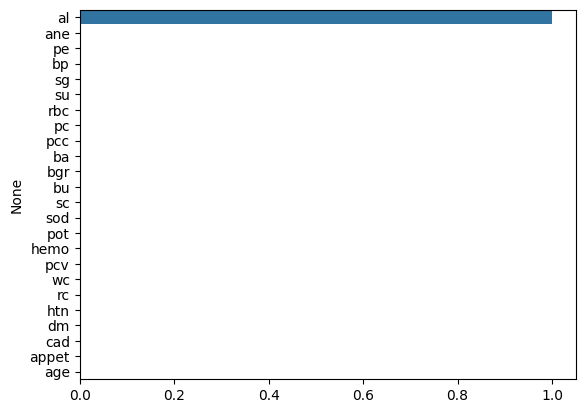
\includegraphics{Seebach_Lily_HW6_files/figure-pdf/cell-24-output-1.png}

From this plot, we can see albumin is the only important variable in
determining an individual's risk of chronic kidney disease according to
the decision tree. Specifically, if albumin is 0, the patient is very
unlikely to have chronic kidney disease, otherwise they likely do have
ckd. This could be due to the sample size and/or test train split. Using
random forests or dropping albumin may reveal other important variables.

\begin{enumerate}
\def\labelenumi{\arabic{enumi}.}
\setcounter{enumi}{13}
\tightlist
\item
  Now split the sub-groups identified in question 7 to improve the
  decision tree accuracy.
\end{enumerate}

\begin{Shaded}
\begin{Highlighting}[]
\NormalTok{xtrain1 }\OperatorTok{=}\NormalTok{ []}
\NormalTok{xtrain2 }\OperatorTok{=}\NormalTok{ []}
\NormalTok{ytrain1 }\OperatorTok{=}\NormalTok{ []}
\NormalTok{ytrain2 }\OperatorTok{=}\NormalTok{ []}
\ControlFlowTok{for}\NormalTok{ i }\KeywordTok{in} \BuiltInTok{range}\NormalTok{(}\BuiltInTok{len}\NormalTok{(X\_train)):}
    \ControlFlowTok{if}\NormalTok{ cluster\_labels\_km1[i] }\OperatorTok{==} \DecValTok{0}\NormalTok{:}
\NormalTok{        xtrain1.append(X\_train.iloc[i])}
\NormalTok{        ytrain1.append(y\_train.iloc[i])}
    \ControlFlowTok{else}\NormalTok{:}
\NormalTok{        xtrain2.append(X\_train.iloc[i])}
\NormalTok{        ytrain2.append(y\_train.iloc[i])}
\NormalTok{xtest1 }\OperatorTok{=}\NormalTok{ []}
\NormalTok{xtest2 }\OperatorTok{=}\NormalTok{ []}
\NormalTok{ytest1 }\OperatorTok{=}\NormalTok{ []}
\NormalTok{ytest2 }\OperatorTok{=}\NormalTok{ []}
\ControlFlowTok{for}\NormalTok{ i }\KeywordTok{in} \BuiltInTok{range}\NormalTok{(}\BuiltInTok{len}\NormalTok{(X\_test)):}
    \ControlFlowTok{if}\NormalTok{ cluster\_labels\_km1[i] }\OperatorTok{==} \DecValTok{0}\NormalTok{:}
\NormalTok{        xtest1.append(X\_test.iloc[i])}
\NormalTok{        ytest1.append(y\_test.iloc[i])}
    \ControlFlowTok{else}\NormalTok{:}
\NormalTok{        xtest2.append(X\_test.iloc[i])}
\NormalTok{        ytest2.append(y\_test.iloc[i])}
\end{Highlighting}
\end{Shaded}

\begin{Shaded}
\begin{Highlighting}[]
\CommentTok{\#\# Using decsion tree}
\NormalTok{x1\_dt }\OperatorTok{=}\NormalTok{ DecisionTreeClassifier(}
\NormalTok{    max\_depth }\OperatorTok{=} \DecValTok{1}\NormalTok{,}
\NormalTok{    random\_state}\OperatorTok{=}\DecValTok{1}
\NormalTok{) }
\NormalTok{x1\_dt.fit(xtrain1,ytrain1)}
\NormalTok{fig, axes }\OperatorTok{=}\NormalTok{ plt.subplots(}
\NormalTok{    nrows }\OperatorTok{=} \DecValTok{1}\NormalTok{,ncols }\OperatorTok{=} \DecValTok{1}\NormalTok{,figsize }\OperatorTok{=}\NormalTok{ (}\DecValTok{4}\NormalTok{,}\DecValTok{4}\NormalTok{), dpi}\OperatorTok{=}\DecValTok{300}
\NormalTok{    )}
\NormalTok{plot\_tree(}
\NormalTok{    x1\_dt, }
\NormalTok{    max\_depth}\OperatorTok{=} \DecValTok{1}\NormalTok{, }
\NormalTok{    feature\_names }\OperatorTok{=}\NormalTok{ X\_train.columns.tolist(), }
\NormalTok{    class\_names}\OperatorTok{=}\NormalTok{[}\StringTok{\textquotesingle{}CKD\textquotesingle{}}\NormalTok{, }\StringTok{\textquotesingle{}No CKD\textquotesingle{}}\NormalTok{], }
\NormalTok{    filled }\OperatorTok{=} \VariableTok{True}
\NormalTok{    )}
\end{Highlighting}
\end{Shaded}

\begin{verbatim}
[Text(0.5, 0.75, 'al <= 1.0\ngini = 0.431\nsamples = 70\nvalue = [22, 48]\nclass = No CKD'),
 Text(0.25, 0.25, 'gini = 0.0\nsamples = 48\nvalue = [0, 48]\nclass = No CKD'),
 Text(0.75, 0.25, 'gini = 0.0\nsamples = 22\nvalue = [22, 0]\nclass = CKD')]
\end{verbatim}

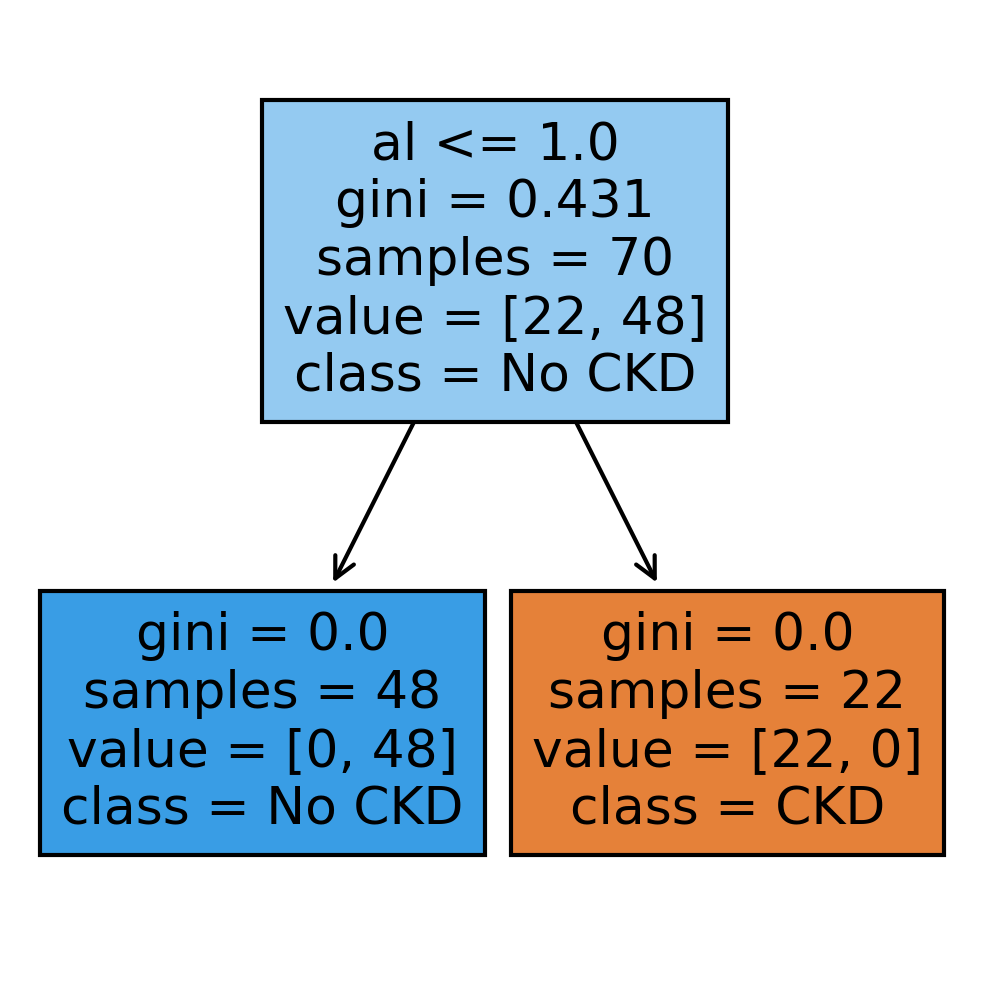
\includegraphics{Seebach_Lily_HW6_files/figure-pdf/cell-26-output-2.png}

\begin{Shaded}
\begin{Highlighting}[]
\NormalTok{x1\_dt.fit(xtrain1, ytrain1)}
\NormalTok{pred }\OperatorTok{=}\NormalTok{ x1\_dt.predict(xtest1)}
\NormalTok{cm }\OperatorTok{=}\NormalTok{ pd.DataFrame(confusion\_matrix(ytest1, pred), index}\OperatorTok{=}\NormalTok{[}\StringTok{\textquotesingle{}No CKD\textquotesingle{}}\NormalTok{, }\StringTok{\textquotesingle{}CKD\textquotesingle{}}\NormalTok{], columns}\OperatorTok{=}\NormalTok{[}\StringTok{\textquotesingle{}No CKD\textquotesingle{}}\NormalTok{, }\StringTok{\textquotesingle{}CKD\textquotesingle{}}\NormalTok{])}
\NormalTok{cm.index.name }\OperatorTok{=} \StringTok{\textquotesingle{}True\textquotesingle{}}
\NormalTok{cm.columns.name }\OperatorTok{=} \StringTok{\textquotesingle{}Predicted\textquotesingle{}}
\NormalTok{sensitivity }\OperatorTok{=}\NormalTok{ cm.iloc[}\DecValTok{1}\NormalTok{,}\DecValTok{1}\NormalTok{]}\OperatorTok{/}\NormalTok{(cm.iloc[}\DecValTok{1}\NormalTok{,}\DecValTok{0}\NormalTok{]}\OperatorTok{+}\NormalTok{cm.iloc[}\DecValTok{1}\NormalTok{,}\DecValTok{1}\NormalTok{])}
\BuiltInTok{print}\NormalTok{(}\StringTok{\textquotesingle{}Sensitivity : \textquotesingle{}}\NormalTok{, sensitivity)}
\BuiltInTok{print}\NormalTok{(}\StringTok{\textquotesingle{}Accuracy : \textquotesingle{}}\NormalTok{, x1\_dt.score(xtest1, ytest1))}
\end{Highlighting}
\end{Shaded}

\begin{verbatim}
Sensitivity :  1.0
Accuracy :  1.0
\end{verbatim}

\begin{Shaded}
\begin{Highlighting}[]
\CommentTok{\#\# Using decsion tree}
\NormalTok{x2\_dt }\OperatorTok{=}\NormalTok{ DecisionTreeClassifier(}
\NormalTok{    max\_depth }\OperatorTok{=} \DecValTok{1}\NormalTok{,}
\NormalTok{    random\_state}\OperatorTok{=}\DecValTok{1}
\NormalTok{) }
\NormalTok{x2\_dt.fit(xtrain2,ytrain2)}
\NormalTok{fig, axes }\OperatorTok{=}\NormalTok{ plt.subplots(}
\NormalTok{    nrows }\OperatorTok{=} \DecValTok{1}\NormalTok{,ncols }\OperatorTok{=} \DecValTok{1}\NormalTok{,figsize }\OperatorTok{=}\NormalTok{ (}\DecValTok{4}\NormalTok{,}\DecValTok{4}\NormalTok{), dpi}\OperatorTok{=}\DecValTok{300}
\NormalTok{    )}
\NormalTok{plot\_tree(}
\NormalTok{    x2\_dt, }
\NormalTok{    max\_depth}\OperatorTok{=} \DecValTok{1}\NormalTok{, }
\NormalTok{    feature\_names }\OperatorTok{=}\NormalTok{ X\_train.columns.tolist(), }
\NormalTok{    class\_names}\OperatorTok{=}\NormalTok{[}\StringTok{\textquotesingle{}CKD\textquotesingle{}}\NormalTok{, }\StringTok{\textquotesingle{}No CKD\textquotesingle{}}\NormalTok{], }
\NormalTok{    filled }\OperatorTok{=} \VariableTok{True}
\NormalTok{    )}
\end{Highlighting}
\end{Shaded}

\begin{verbatim}
[Text(0.5, 0.75, 'pcv <= 38.0\ngini = 0.32\nsamples = 40\nvalue = [8, 32]\nclass = No CKD'),
 Text(0.25, 0.25, 'gini = 0.0\nsamples = 8\nvalue = [8, 0]\nclass = CKD'),
 Text(0.75, 0.25, 'gini = 0.0\nsamples = 32\nvalue = [0, 32]\nclass = No CKD')]
\end{verbatim}

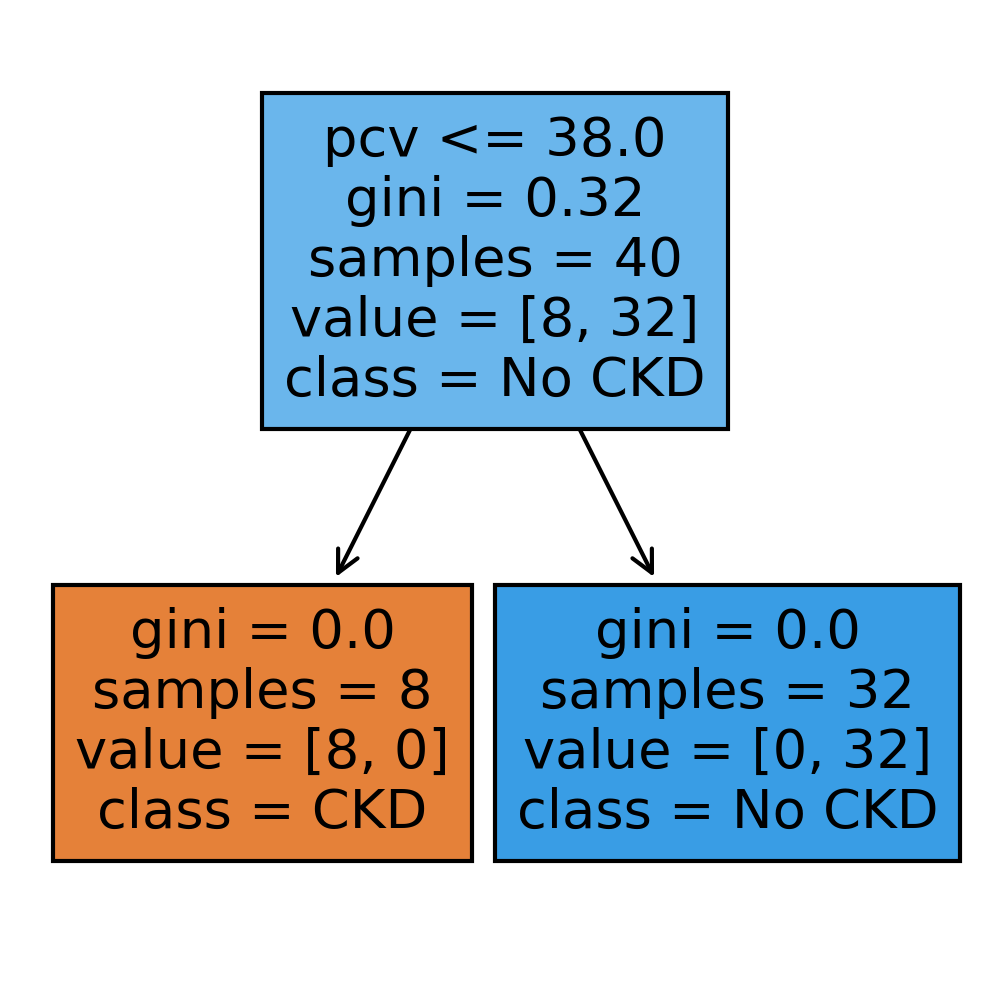
\includegraphics{Seebach_Lily_HW6_files/figure-pdf/cell-28-output-2.png}

\begin{Shaded}
\begin{Highlighting}[]
\NormalTok{x2\_dt.fit(xtrain2, ytrain2)}
\NormalTok{pred }\OperatorTok{=}\NormalTok{ x2\_dt.predict(xtest2)}
\NormalTok{cm }\OperatorTok{=}\NormalTok{ pd.DataFrame(confusion\_matrix(ytest2, pred), index}\OperatorTok{=}\NormalTok{[}\StringTok{\textquotesingle{}No CKD\textquotesingle{}}\NormalTok{, }\StringTok{\textquotesingle{}CKD\textquotesingle{}}\NormalTok{], columns}\OperatorTok{=}\NormalTok{[}\StringTok{\textquotesingle{}No CKD\textquotesingle{}}\NormalTok{, }\StringTok{\textquotesingle{}CKD\textquotesingle{}}\NormalTok{])}
\NormalTok{cm.index.name }\OperatorTok{=} \StringTok{\textquotesingle{}True\textquotesingle{}}
\NormalTok{cm.columns.name }\OperatorTok{=} \StringTok{\textquotesingle{}Predicted\textquotesingle{}}
\NormalTok{sensitivity }\OperatorTok{=}\NormalTok{ cm.iloc[}\DecValTok{1}\NormalTok{,}\DecValTok{1}\NormalTok{]}\OperatorTok{/}\NormalTok{(cm.iloc[}\DecValTok{1}\NormalTok{,}\DecValTok{0}\NormalTok{]}\OperatorTok{+}\NormalTok{cm.iloc[}\DecValTok{1}\NormalTok{,}\DecValTok{1}\NormalTok{])}
\BuiltInTok{print}\NormalTok{(}\StringTok{\textquotesingle{}Sensitivity : \textquotesingle{}}\NormalTok{, sensitivity)}
\BuiltInTok{print}\NormalTok{(}\StringTok{\textquotesingle{}Accuracy : \textquotesingle{}}\NormalTok{, x2\_dt.score(xtest2, ytest2))}
\end{Highlighting}
\end{Shaded}

\begin{verbatim}
Sensitivity :  1.0
Accuracy :  1.0
\end{verbatim}

The accuracy for the first and second subgroup is 1. In both question 12
and 14, the sensitivity is one. Therefore, the accuracy is slightly
improved after first splitting the data based on K-means clustering,
with K=2. However, sensitivity remains unchanged.

\subsection*{Bibliography}\label{bibliography}
\addcontentsline{toc}{subsection}{Bibliography}

\phantomsection\label{refs}
\begin{CSLReferences}{1}{0}
\bibitem[\citeproctext]{ref-misc_chronic_kidney_disease_336}
Rubini, L., Soundarapandian P., and P. Eswaran. 2015. {``{Chronic Kidney
Disease}.''} UCI Machine Learning Repository.

\end{CSLReferences}



\end{document}
